\documentclass[a4paper,12pt,italian]{report}

\usepackage[italian]{babel}             %Nomi italiani
\usepackage[latin1]{inputenc}           %Lettere accentate
\usepackage{graphicx,color}                   %Inclusione delle figure
\usepackage{url}

%\usepackage{shading}
%\usepackage{moreverb}                   %Enhanced verbatim (per le linee di codice)
%\usepackage[isu,footnotesize]{caption}  %Caption piccole e indentate
%\usepackage{setspace}                   %Interlinea
\usepackage[hang,footnotesize]{subfigure} %Inserimento di subfigures
\usepackage[subfigure,titles]{tocloft}
\usepackage{listings}
\lstset{language=C++}

%%%%%%%%%%%%%%%%%%%%%%%%%%%%  Nuovi ambienti floating  %%%%%%%%%%%%%%%%%%%%%%%%%%%
%\usepackage{float}
%\floatstyle{ruled}
%\newfloat{program}{tbp}{lol}[chapter]
%\floatname{program}{\programname}

%%%%%%%%%%%%%%%%%%%%%%%%%%%%  HighLight sorgenti: ambiente lgrind %%%%%%%%%%%%%%%%%%%%%%%%%%%

%%%%%%%%%%%%%%%%%%%%%%%%%%%%  Headings & Footings %%%%%%%%%%%%%%%%%%%%%%%%%%%

\usepackage{fancyhdr} \pagestyle{fancy}%
\makeatletter
\renewcommand{\chaptermark}[1]{\markboth{\footnotesize \thechapter.\ #1}{}}%
%\renewcommand{\sectionmark}[1]{\markright{\MakeUppercase \footnotesize \thesection.\ #1}{}}%
\makeatother

\fancyhf{}                              %Elimino header e footer di default
\fancyhead[R]{\thepage}      %Imposto l'header sinistro con il nome del capitolo
\fancyhead[L]{\bfseries \leftmark}                 %Imposto l'header destro con il numero di pagina
%\fancyhead[OR]{\bfseries \leftmark}      %Imposto l'header sinistro con il nome del capitolo
%\fancyhead[OL]{\thepage}                 %Imposto l'header destro con il numero di pagina
%\fancyhead[EL]{\bfseries \rightmark}      
%\fancyhead[ER]{\thepage}             

\headheight 16pt                        %Altezza dell'header per evitare overfull box
% ridefinisco lo stile plain per le pagine di inizio capitolo
\fancypagestyle{plain}{%
  \fancyhf{}                            %Elimino header e footer di default
  \fancyfoot[C]{\thepage}               %Imposto il numero di pagina al centro del footer
  \renewcommand{\headrulewidth}{0pt}    %Nessuna linea sull'header
  \renewcommand{\footrulewidth}{0pt}    %Nessuna linea sul footer
}
%%%%%%%%%%%%%%%%%%%%%%%%%%%%%%%%%%%%%%%%%%%%%%%%%%%%%%%%%%%%%%%%%%%%%%%%%%%%%%%%%

%\usepackage[nolineno,noindent]{lgrind} %[noindent,nolineno,procnames,noprocindex,fussy,norules,nolineno,leftno,lineno5]
%\newcommand{\programinput}[1]{\begin{spacing}{1} \footnotesize \verbatiminput{#1} \end{spacing}}
%\newcommand{\lgrindinput}[1]{
%    \begin{lgrind}
%      \footnotesize
%      \input{#1}
%    \end{lgrind}
%}
\newcommand{\cod}{\texttt}

%\newcommand\ttpfamily{\fontfamily{ccr}\selectfont\footnotesize}
%\usepackage{concrete}
\usepackage[T1]{fontenc}
\DeclareFontFamily{T1}{ttp}{}
%\usepackage{beton}
\usepackage{t1enc}

% Definizioni font per il pacchetto lgrind
%\def\CMfont{\sffamily\itshape}
%\def\KWfont{\sffamily\bfseries}
%\def\VRfont{\ttfamily}
%\def\BGfont{\ttfamily}

\newcommand{\method}[4]{
  \begin{raggedright}
    \begin{tabular}{p{.40\textwidth}p{.23\textwidth}p{.23\textwidth}}
      \cod{#1()} & \cod{#2} & \cod{#3}\\
      \multicolumn{3}{p{.9\textwidth}}{#4}\\
    \end{tabular}
    \bigskip
  \end{raggedright}
}

\newcommand{\methodsheader}{
  \bigskip
  \begin{raggedright}
    \begin{tabular}{p{.40\textwidth}p{.23\textwidth}p{.23\textwidth}}
      Nome & Param.~Ingr. & Param.~Usc.\\
      \hline
    \end{tabular}
  \end{raggedright}  
  \nolinebreak
  
%Don't erase the above empty line
}

\newenvironment{methodslist}
  {
    %\sffamily
    \methodsheader
    \nopagebreak
  }
  {
    %\rmfamily
  }

\renewcommand{\emptyset}{$\phi$}
\def\sectionname{Esercizio}
\newcommand{\cfr}[1]{\seename~�\ref{#1}}
\def\version{V0.88}

%\newcommand{\inputprogram}[2]{
%  \subsubsection*{\textcolor[gray]{.4}{\sffamily File \cod{#1}}}
%  \lgrindinput{#2}
%}

\lstnewenvironment{codequote}
  {
    \footnotesize
  }
  {
  }

\newcommand{\inputmodule}[2]{
  {\bigskip
   \center
    \subsubsection*{\textcolor[gray]{.4}{\sffamily \framebox{File \cod{#1}}}}
  }
  \scriptsize
  \lstinputlisting{#2}
  \normalsize  
  \lstset{numbers=none} %disable lines numbering
}

\newcommand{\enablelstnum}{
  \lstset{numbers=left, numberstyle=\tiny, stepnumber=1, numbersep=5pt}
}

\newcommand{\inputprogram}[1]{
  \scriptsize
  \lstinputlisting{#1}
  \normalsize  
  \lstset{numbers=none} %disable lines numbering
}

\newcommand{\exercise}[1]{
  \section{#1}
  %\newline
  {
  \hfill
  \footnotesize\sffamily
  \textcolor[gray]{.4}{Soluzione a pag.~\pageref{Sol:#1}}
  \label{Ex:#1}
  \newline
  }	
}

\newcommand{\solution}[0]{\subsection*{Soluzione}}
\newcommand{\thesolution}[1]{
  \section{#1}
  %\newline
  {
  \hfill
  \footnotesize\sffamily
  \textcolor[gray]{.4}{Traccia a pag.~\pageref{Ex:#1}}
  \label{Sol:#1}
  \newline
  }
}

%Fix small space for numbers in the TOC
%\makeatletter\renewcommand{\l@section}{\@dottedtocline{1}{1.5em}{3.3em}}\makeatother

% define the title
\makeatletter
\def\thickhrulefill{\leavevmode \leaders \hrule height 1pt\hfill \kern \z@}
\renewcommand{\maketitle}{\begin{titlepage}%
    \let\footnotesize\small
    \let\footnoterule\relax
    \parindent \z@
    \reset@font
    \null\vfil
    \vspace{3cm}
    \begin{flushleft}
      \huge \@title \normalsize \hfill \version
    \end{flushleft}
    \par
    \hrule height 4pt
    \par
    \begin{flushright}
      \LARGE \@author \par
    \end{flushright}
    \vfill
    Copyright \copyright  2006-2009 Marcello Esposito. Permission is granted to copy,
    distribute and/or modify this document under the terms of the GNU Free Documentation License,
    Version 1.2 or any later version published by the Free Software Foundation; with no Invariant
    Sections, no Front-Cover Texts, and no Back-Cover Texts. A copy of the license is included
    in the section entitled "GNU Free Documentation License".
  \end{titlepage}%
  \setcounter{footnote}{0}%
}

\makeatother
\author{Marcello Esposito}
\title{51 Esercizi di C++}
\date{2009}

\begin{document}
%Tune space between numbers and titles in toc (uses package tocloft)
\addtolength{\cftchapnumwidth}{.5\cftchapnumwidth}
\addtolength{\cftsecnumwidth}{.5\cftsecnumwidth}

\maketitle
\tableofcontents
\clearpage
%\listoffigures
%\clearpage

\markboth{Prefazione}{Prefazione}
\chapter*{Prefazione}
\addcontentsline{toc}{chapter}{\numberline{}Prefazione}%
Gli esercizi presentati in questo eserciziario sono stati originariamente assegnati ad un corso universitario di \emph{Programmazione I} al secondo e terzo anno di Ingegneria delle Telecomunicazioni. Il corso richiedeva di realizzarne le soluzioni in linguaggio C++. Successivamente sono tradotti in linguaggio Java dal testo \emph{50 esercizi di C++ con soluzioni}~\cite{EserciziCpp}.

Il corso aveva lo scopo di introdurre alla programmazione orientata agli oggetti. Una rilevante parte del programma affrontava lo studio dei tipi di dati astratti, con particolare enfasi sulle strutture dati di tipo contenitore, stressandone i concetti di incapsulamento ed interfaccia. Gli esercizi dedicati all'approfondimento di questi concetti sono stati raccolti in questo eserciziario, insieme con le relative soluzioni.

\section*{A chi � rivolto questo testo}
Gli studenti che approcciano allo studio del linguaggio Java, in occasione di corsi di studi superiori, troveranno utile studiare e risolvere gli esercizi contenuti in questo testo. Se da un lato questi favoriscono l'acquisizione delle ricorrenti tecniche legate alla realizzazione ed all'uso di contenitori, dall'altro rappresentano un pretesto per mettere in pratica approcci algoritmici alla risoluzione di problemi pi� generici. Il libro si focalizza sulla progettazione degli algoritmi pi� che sulla sintassi e sull'uso esteso dello specifico linguaggio.

Non essendo questo un libro di teoria, lo studio di uno dei numerosi testi dedicati alle nozioni della programmazione, alle regole ed alla sintassi del linguaggio Java, risulta propedeutico. Un diffuso testo orientato all'apprendimento del linguaggio �~\cite{Eckel}.

\section*{La struttura degli esercizi}
Questo eserciziario contiene differenti tipologie di esercizi: alcuni richiedono la realizzazione di una struttura dati di tipo contenitore, mediante uso del costrutto \cod{class} del linguaggio, fornendo allo studente la specifica in forma di interfaccia dei classici metodi di cui tali strutture sono dotate (aggiunta di un elemento, conteggio degli elementi, svuotamento, visita, etc.). Altri esercizi, basandosi sulle suddette implementazioni, richiedono la realizzazione di funzionalit� finalizzate ad effettuare particolari elaborazioni sugli elementi contenuti (per esempio inserimenti o eliminazioni condizionate, somme, spostamenti, conteggi, etc.). Infine, alcuni esercizi richiedono la realizzazione di strutture dedicate a risolvere specifici problemi, e quindi prive dei classici requisiti di generalit�.

Per ogni metodo da implementare, una traccia fornisce le seguenti informazioni:
\begin{itemize}
  \item il nome del metodo;
  \item l'insieme dei parametri di ingresso;
  \item l'insieme dei parametri di uscita;
  \item la descrizione della funzionalit� che il metodo deve realizzare.
\end{itemize}

Per esempio, la specifica di un ipotetico metodo di eliminazione di elementi da una lista, potrebbe apparire come segue.

\bigskip
  \sffamily
  \begin{methodslist}
  \method{elimina}{int}{int}{
  Elimina dalla struttura tutte le occorrenze dell'elemento specificato dal parametro di ingresso. Restituisce il numero delle eliminazioni effettuate.
  }
  \end{methodslist}
  \rmfamily  
\bigskip

Nel caso in cui l'insieme dei parametri di ingresso e/o di uscita fosse vuoto, si utilizzer� il simbolo~``\emptyset''. Talvolta pu� accadere che nella descrizione del funzionamento del metodo non si prenda in considerazione la totalit� dei casi che possono verificarsi (pre-condizioni), limitandosi a descrivere il comportamento del metodo nei casi d'uso pi� comuni. In questo caso, il programmatore pu� scegliere arbitrariamente un comportamento per tutti i casi non esplicitamente considerati.

Per quanto riguarda le strategie di gestione della memoria, la realizzazione delle strutture dati pu� basarsi su un approccio di tipo statico (uso di vettori allocati sullo stack) oppure dinamico (realizzazione di strutture concatenate con puntatori ed allocate nell'heap mediante costrutto \cod{new}). Questa scelta, in alcuni casi, � lasciata alla sensibilit� dello studente.

Per ognuno degli esercizi, oltre alla traccia, si fornisce la soluzione consistente nell'implementazione dei metodi conformi all'interfaccia specificata dalla traccia. Nel caso in cui la traccia richieda di realizzare una struttura dati completa (e non solo i metodi basati su di essa, nella soluzione viene anche fornito un modulo di test (di solito rappresentato dalla funzione \cod{main()} della classe \cod{Main}) utile esclusivamente al collaudo delle funzionalit� della classe.

Al fine di preservare una maggiore generalit� delle strutture dati realizzate, un esplicito requisito comune a tutti gli esercizi consiste nel vietare l'uso dei meccanismi di I/O nell'implementazione dei metodi della classe. La responsabilit� di prelevare i dati da tastiera e mostrare i risultati sulla console viene pertanto delegata al modulo di test, mentre la classe resta indipendente dalla tecnologia utilizzata per l'interfacciamento grafico con l'utente. Pertanto, anzich� stampare direttamente, i metodi di visita delle strutture contenitore (per es. stampa degli elementi di una lista) costruiscono e restituiscono una stringa contenente l'insieme degli elementi. Allo scopo utilizzano la classe \cod{StringBuilder} della libreria standard \cod{java.lang}, che consente proprio la composizione incrementale ed efficiente di grosse stringhe di testo mediante uso del metodo \cod{append()}. Non sar� necessario quindi modificare la classe nel caso in cui, in futuro, si decidesse di utilizzare una diversa interfaccia grafica (es. SWT, HTML, ecc.) per acquisire i dati e mostrare i risultati delle elaborazioni. 

%Un'unica deroga a questa regola � relativa al metodo di visita delle strutture (di solito contrassegnato dal nome \cod{Stampa()}): il concetto di \emph{iteratore}, utile ad astrarre l'attraversamento di una struttura contenitore, non � di solito noto agli studenti di un corso di base. Il lettore interessato pu� fare riferimento alla Standard Template Library (STL)~\cite{STL}, peraltro di notevole utilit� in reali contesti di sviluppo software. Per le operazioni di I/O si utilizzano le funzionalit� messe a disposizione dalla libreria standard \cod{iostream}, ed in particolare dai suoi oggetti \cod{cin} e \cod{cout}.

\section*{Compilare i sorgenti}
%\addcontentsline{toc}{section}{\numberline{}Compilare i sorgenti}%
Tutti i sorgenti presentati sono stati compilati con l'ambiente di sviluppo integrato \emph{Eclipse} per Java, nella sua versione \emph{Luna Service Release 2 (4.4.2)}. L'estrema portabilit� del linguaggio Java non dovrebbe rendere complicata la compilazione su altri ambienti di sviluppo.

\section*{Uno sguardo al futuro}
Quelli che alla fine di questo eserciziario penseranno: \emph{``S�, e allora?''}, probabilmente sono pronti per affrontare uno studio pi� approfondito della programmazione, che non si esaurisce con il possesso delle nozioni sulla progettazione di generici algoritmi e un'infarinatura sulle basi del linguaggio. Tra un individuo che conosca un linguaggio di programmazione ed un programmatore esperto c'� un differenza analoga a quella che esiste tra un individuo che sappia scrivere ed uno scrittore. Un buon programmatore non � quello che sa \emph{affrontare} la complessit�, ma quello che sa \emph{dominarla}. Certamente la conoscenza della sintassi del linguaggio � un primo passo indispensabile, ma chi vuole approfondire questa affascinante materia non pu� fare a meno di acquisire le nozioni della progettazione, le buone prassi per la stesura del codice e gli strumenti forniti dalle librerie standard oggi disponibili. \`{E} solo attraverso questa strada che diviene possibile scrivere applicazioni non banali, preservandone le caratteristiche di comprensibilit�, estensibilit�, manutenibilit�, correttezza e, in una sola parola, di \emph{qualit�}. Programmare utilizzando l'incapsulamento, il polimorfismo, i meccanismi delle eccezioni, delle asserzioni, dei generics, le numerose librerie pi� o meno standard, significa disporre di strumenti semanticamente molto potenti, oltre che ben consolidati; significa delegare al compilatore lo svolgimento di una serie di operazioni e di controlli che, in alternativa, peserebbero sulle spalle del programmatore, oppure non verrebbero messi in essere affatto.

Nell'apprendere le nozioni della progettazione e le buone prassi per la stesura del codice, ascoltare cosa hanno da dirci `i giganti' al proposito, pu� servire molto. A questo scopo non si pu� fare a meno di citare dei testi disponibili in letteratura, universalmente considerati dei classici.

\emph{Design Patterns}~\cite{GoF} � probabilmente il pi� bel testo mai scritto nell'ambito della progettazione software, considerando anche le profonde ripercussioni che esso ha poi avuto sul concetto di buona progettazione software orientata agli oggetti, tanto da essere ancora oggi il libro di gran lunga pi� citato nel suo genere. In questo testo gli autori introducono il concetto di \emph{pattern progettuale software} (\emph{design pattern}); ad un livello di astrazione superiore a quello di qualsiasi linguaggio di programmazione, presentano poi 55 soluzioni a problemi comuni nell'ambito della progettazione, con esempi in linguaggio C++. Ne esistono varie versioni declinate nel linguaggio Java. Imperdibile.

A livello professionale, � molto utile approfondire altri patterns consolidati. Un importante aspetto riguarda l'interfacciamento delle applicazioni con le basi di dati relazionali. Queste ultime, progettate prima della vasta diffusione della programmazione orientata agli oggetti, male si adattano ad interagire con le moderne applicazioni. Per questo si sono recentemente sviluppati prodotti classificati come \emph{object/relational mappers}, il cui uso consapevole migliora notevolmente le caratteristiche di correttezza, modularit�, portabilit�, efficienza di un'applicazione transazionale. Chi invece preferisse un approccio pi� radicale, estremamente promettente ed in fase di rapida diffusione, pu� approfondire l'uso dei \emph{database documentali}, tra i quali attualmente spicca MongoDB per numero di installazioni e tasso di crescita. Un altro interessante pattern \emph{trasversale} � quello della \emph{dependency-injection}, che naturalmente instrada ad uno sviluppo delle classi pulito, essenziale, modulare, nel rispetto dei principali parametri di qualit� del software. Chi fosse interessato pu� approfondire la tematica cercando informazioni sui cinque principi della programmazione SOLID.

\section*{Dove trovare questo eserciziario}
Questo eserciziario � distribuito sotto licenza GNU Free Documentation License (vedi \appendixname~\ref{label:fdl}) all'indirizzo \url{http://esercizicpp.sourceforge.net}. Dal sito � possibile prelevare l'ultima versione disponibile, accedere ai forum dedicati ai lettori ed iscriversi alla mailing-list informativa.

\section*{Contattare l'autore}
%\addcontentsline{toc}{section}{\numberline{}Contattare l'autore}%
Commenti, suggerimenti e segnalazioni sono graditi. L'autore pu� essere contattato al seguente indirizzo e-mail: \url{esposito.marce@gmail.com}

\part{Esercizi}

\renewcommand{\thechapter}{EL}
\chapter{Esercizi su liste}
\exercise{Lista Semplicemente Collegata}
Si realizzi la struttura dati \cod{Lista} secondo l'implementazione della lista semplicemente collegata (ogni elemento punta al successivo). Il tipo degli elementi contenuti sia uguale al tipo \cod{int} del linguaggio. La lista sia dotata dei metodi riportati di seguito.

\begin{methodslist}
\method{Lista}{\emptyset}{\emptyset} {
 Costruttore senza parametri.
}

\method{Lista}{Lista}{\emptyset} {
  Costruttore di copia.
}

\method{inserisci}{int}{\emptyset} {
  Inserimento in testa alla lista.
}

\method{numeroElementi}{\emptyset}{int} {
  Restituisce il numero degli elementi contenuti nella lista.
}

\method{svuota}{\emptyset}{\emptyset} {
  Svuota la lista.
}

\method{elimina}{int}{\emptyset} {
  Elimina un elemento dalla lista, se presente.
}

\method{toString}{\emptyset}{String} {
  Restituisce in forma testuale la rappresentazione della struttura costituita da tutti gli elementi contenuti nella lista.
}

\method{ricerca}{int}{boolean} {
  Predicato indicante la presenta di un elemento.
}

Si realizzi una classe \cod{Main} dotata del metodo \cod{public static void main()} che permetta di effettuare il collaudo della struttura dati realizzata.

\end{methodslist}
\exercise{Somma Elementi}
Dotare la classe \cod{Lista} (\cfr{Ex:Lista Semplicemente Collegata}) del metodo \cod{Somma()} secondo la seguente specifica.

\begin{methodslist}

\method{Somma}{\emptyset}{TElem} {
Restituisce la somma degli elementi presenti nella lista.
}

\end{methodslist}
\exercise{Coda Pari}
Dotare la classe \cod{Lista} (\cfr{Ex:Lista Semplicemente Collegata}) del metodo \cod{CodaPari()}, secondo la seguente interfaccia.

\begin{methodslist}

\method{CodaPari}{\emptyset}{bool} {
Restituisce \cod{true} se l'elemento in coda � pari, \cod{false} altrimenti.
}

\end{methodslist}
\exercise{Min e Max}
Dotare la classe \cod{Lista} (\cfr{Ex:Lista Semplicemente Collegata}) del metodo \cod{MinMax()} secondo la seguente specifica.

\begin{methodslist}

\method{MinMax}{\emptyset}{TElem,TElem} {
Restituisce gli elementi minimo e massimo all'interno della lista. In caso di lista vuota l'uscita di questo metodo � non specificata.
}

\end{methodslist}

\exercise{Lista Statica}
Si realizzi la struttura dati \cod{Lista} secondo un approccio all'allocazione della memoria di tipo statico. Il tipo \cod{TElem} degli elementi contenuti sia uguale al tipo \cod{int} del linguaggio. La lista sia dotata dei metodi riportati di seguito.

\begin{methodslist}

\method{Lista}{\emptyset}{\emptyset}{
Costruttore.
}

\method{\~{}Lista}{\emptyset}{\emptyset}{
Distruttore.
}

\method{InserisciInCoda}{TElem}{\emptyset}{
Inserisce un elemento in coda alla lista.
}

\method{Svuota}{\emptyset}{\emptyset}{
Svuota la lista.
}

\method{Count}{\emptyset}{int}{
Restituisce il numero degli elementi contenuti nella lista.
}

\method{Stampa}{\emptyset}{\emptyset}{
Stampa sullo standard output tutti gli elementi contenuti nella lista.
}

\end{methodslist}

L'unico metodo della classe Lista che pu� utilizzare lo standard-output (\cod{cout}) � il metodo \cod{Stampa()}. Gli altri metodi (pubblici, privati o protetti) non possono fare uso delle funzionalit� di stampa.
\exercise{\`{E} Ordinata}
Dotare la classe \cod{Lista} (\cfr{Ex:Lista Statica}) del metodo \cod{eOrdinata()}, secondo la seguente interfaccia.

\begin{methodslist}

\method{eOrdinata}{\emptyset}{boolean} {
Restituisce \cod{true} se la lista � ordinata secondo la relazione di ordinamento crescente per gli interi, \cod{false} altrimenti.
}

\end{methodslist}
\exercise{Elimina Tutti}
Dotare la classe \cod{Lista} (\cfr{Ex:Lista Statica}) del metodo \cod{eliminaTutti()}, secondo la seguente interfaccia.

\begin{methodslist}

\method{eliminaTutti}{int}{int} {
Elimina tutte le occorrenze dell'elemento specificato presenti nella lista. Restituisce il numero di occorrenze eliminate.
}

\end{methodslist}
\exercise{Elimina Ultimi}
Dotare la classe \cod{Lista} (\cfr{Ex:Lista Semplicemente Collegata}) dei metodi le cui interfacce sono riportate di seguito.

\begin{methodslist}

\method{EliminaUltimi}{unsigned int}{unsigned int} {
Elimina dalla lista gli ultimi \cod{n} elementi, con \cod{n} pari al valore del parametro di ingresso. Il valore restituito � pari al numero di elementi effettivamente eliminati dalla lista.
}

\method{LasciaPrimi}{unsigned int}{unsigned int} {
Elimina dalla lista tutti gli elementi tranne i primi \cod{n}, con \cod{n} pari al valore del parametro di ingresso. Il valore restituito � pari al numero di elementi effettivamente eliminati dalla lista.
}

\end{methodslist}
\exercise{Somma Coda}
Dotare la classe \cod{Lista} (\cfr{Ex:Lista Semplicemente Collegata}) del metodo \cod{sommaCoda()}, secondo la seguente interfaccia.

\begin{methodslist}

\method{sommaCoda}{\emptyset}{\emptyset} {
Somma a tutti gli elementi della lista il valore dell'elemento di coda.
}

\end{methodslist}
\exercise{Sposta Testa in Coda}
Dotare la classe \cod{Lista} (\cfr{Ex:Lista Semplicemente Collegata}) del metodo \cod{spostaTestaInCoda()}, secondo la seguente interfaccia.

\begin{methodslist}

\method{spostaTestaInCoda}{\emptyset}{boolean} {
Sposta in coda alla lista l'elemento di testa. Il metodo restituisce \cod{true} se lo spostamento � effettuato, \cod{false} altrimenti.
}

\end{methodslist}
\exercise{Elimina Pari e Dispari}
Dotare la classe \cod{Lista} (\cfr{Ex:Lista Semplicemente Collegata}) dei metodi \cod{EliminaElPostoPari()} ed \cod{EliminaElPostoDispari()}, secondo la seguente interfaccia.

\begin{methodslist}

\method{EliminaElPostoPari}{\emptyset}{unsigned int} {
Elimina dalla lista tutti gli elementi di posto pari (0, 2, 4, ...). Restituisce il numero di elementi eliminati.
}

\method{EliminaElPostoDispari}{\emptyset}{unsigned int} {
Elimina dalla lista tutti gli elementi di posto dispari (1, 3, 5, ...). Restituisce il numero di elementi eliminati.
}

\end{methodslist}
\exercise{Lista Doppiamente Collegata}
Si realizzi in linguaggio C++ il tipo di dato astratto \cod{Lista} mediante uso del costrutto \cod{class} del linguaggio. L'implementazione deve essere realizzata mediante puntatori ed allocazione dinamica della memoria secondo l'approccio di lista doppiamente collegata. Ogni elemento, cio�, punta contemporaneamente al precedente ed al successivo (vedi \figurename~\ref{fig:ListaDoppiamenteCollegata}). Gli elementi della lista siano uguali al tipo \cod{int} del linguaggio.

\begin{figure}
  \center
	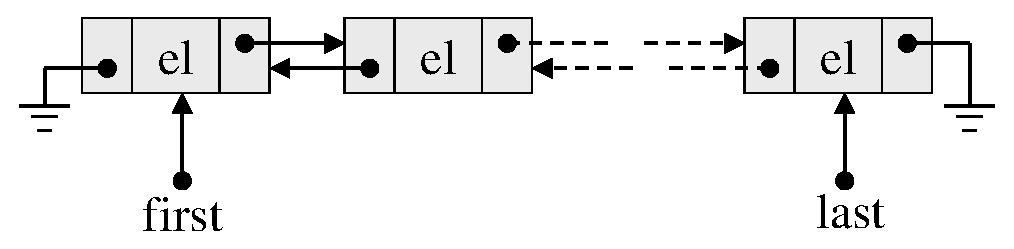
\includegraphics[width=.7\textwidth]{Esercizi/ListaDoppiamenteCollegata/Lista.eps}
	\caption{Struttura della lista doppiamente collegata}
	\label{fig:ListaDoppiamenteCollegata}
\end{figure}
        
Di seguito � riportata la specifica dei metodi pubblici da implementare per la classe \cod{Lista}.

\begin{methodslist}

\method{Lista}{\emptyset}{\emptyset} {
Costruttore.
}

\method{inserisci}{int}{\emptyset} {
Inserisce un elemento in coda alla lista.
}

\method{svuota}{\emptyset}{\emptyset} {
Svuota la lista.
}

\method{count}{\emptyset}{int} {
Conta gli elementi contenuti nella lista.
}

\method{stampaDiretta}{\emptyset}{String} {
Restituisce una stringa contenente tutti gli elementi della lista, dall'elemento di testa all'elemento di coda.
}

\method{stampaInversa}{\emptyset}{String} {
Restituisce una stringa contenente tutti gli elementi della lista, dall'elemento di coda all'elemento di testa.
}

\method{stampaAlternata}{\emptyset}{String} {
Restituisce una stringa con il contenuto della lista nel seguente ordine: primo elemento, ultimo elemento, secondo elemento, penultimo elemento, terzo elemento, terzultimo elemento...
}

Nessun metodo della classe Lista pu� utilizzare le funzionalit� di stampa (\cod{System.out}).

Si realizzi una funzione \cod{main()} che permetta di effettuare il collaudo della struttura dati realizzata.

\end{methodslist}
\exercise{Ribalta}
Dotare la classe \cod{Lista} (\cfr{Ex:Lista Semplicemente Collegata}) del metodo \cod{Ribalta()} secondo la seguente specifica.

\begin{methodslist}

\method{Ribalta}{\emptyset}{\emptyset} {
Ribalta la posizione di tutti gli elementi della lista. Alla chiamata di tale metodo il primo elemento diventa l'ultimo, il secondo diventa il penultimo\ldots\ l'ultimo diventa il primo.
}

\end{methodslist}

\renewcommand{\thechapter}{EA}
\chapter{Esercizi su alberi binari}
\exercise{Albero Binario}
Realizzare la classe \cod{AlberoBinario}. Il tipo \cod{TElem} dei suoi elementi sia il tipo \cod{int} e gli elementi risultino ordinati secondo la relazione di ordinamento crescente per gli interi. L'implementazione di tutti i metodi sia basata su appositi metodi ricorsivi. L'interfaccia della classe sia la seguente.
  
\begin{methodslist}

\method{AlberoBinario}{\emptyset}{\emptyset} {
Costruttore della struttura.
}

\method{AlberoBinario}{AlberoBinario}{\emptyset} {
Costruttore di copia.
}

\method{\~{}AlberoBinario}{\emptyset}{\emptyset} {
Distruttore della struttura.
}

\method{AggiungiElem}{TElem}{\emptyset} {
Metodo di aggiunta di un elemento all'albero.
}

\method{InAlb}{TElem}{bool} {
Ricerca un elemento nell'albero. Restituisce \cod{true} nel caso in cui l'elemento specificato sia presente nell'albero, \cod{false} altrimenti.
}

\method{Elimina}{TElem}{\emptyset} {
Elimina l'elemento specificato dall'albero.
}

\method{Svuota}{\emptyset}{\emptyset} {
Svuota la struttura.
}

\method{PreOrdine}{\emptyset}{\emptyset} {
Effettua una visita in pre-ordine dell'albero, stampando tutti gli elementi sullo standard output.
}

\method{PostOrdine}{\emptyset}{\emptyset} {
Effettua una visita in post-ordine dell'albero, stampando tutti gli elementi sullo standard output.
}

\method{InOrdine}{\emptyset}{\emptyset} {
Effettua una visita in ordine dell'albero, stampando tutti gli elementi sullo standard output.
}

Gli unici metodi della classe \cod{AlberoBinario} che possono utilizzare direttamente o indirettamente lo standard-output (\cod{cout}) sono i metodi di visita dell'albero (\cod{InOrdine()}, \cod{PreOrdine()}, \cod{PostOrdine()} e gli eventuali metodi privati di supporto da questi invocati). Gli altri metodi (pubblici, privati o protetti) non possono fare uso delle funzionalit� di stampa.

Si realizzi una funzione \cod{main()} che permetta di effettuare il collaudo della struttura dati realizzata.

\end{methodslist}
\exercise{Numero Elementi}
Dotare la classe \cod{AlberoBinario} (\cfr{Ex:Albero Binario}) del metodo \cod{numElem()} secondo la seguente specifica.

\begin{methodslist}

\method{numElem}{\emptyset}{int} {
  Restituisce il numero degli elementi presenti nell'albero.
}

\end{methodslist}
\exercise{Occorrenze}
Dotare la classe \cod{AlberoBinario} (\cfr{Ex:Albero Binario}) del metodo \cod{occorrenze()}, secondo la seguente interfaccia.

\begin{methodslist}

\method{occorrenze}{int}{int} {
Restituisce le occorrenze dell'elemento specificato nell'albero.
}

\end{methodslist}
\exercise{Occorrenza Massima}
Modificare la classe \cod{AlberoBinario} (\cfr{Ex:Albero Binario}) per prevedere un'occorrenza massima degli elementi in esso inseriti. Pi� precisamente, il costruttore deve accettare come parametro di ingresso un numero intero positivo (per es. \cod{occMax}); l'inserimento di un nuovo elemento nell'albero deve andare a buon fine solo se tale elemento � presente con occorrenza minore di \cod{occMax}.

Di seguito � riportata la specifica dei due metodi pubblici da implementare per la classe \cod{AlberoBinario}.

\begin{methodslist}

\method{AlberoBinario}{int}{\emptyset} {
Costruttore con parametro di ingresso di tipo intero non negativo. Il parametro di ingresso rappresenta l'occorrenza massima con cui gli elementi potranno essere presenti nell'albero.
}

\method{aggiungiElem}{int}{boolean}{
Inserisce l'elemento specificato nell'albero solo se esso � presente con occorrenza minore dell'occorrenza massima specificata nel costruttore.

Il metodo restituisce \cod{true} o \cod{false} a seconda che l'inserimento sia avvenuto o meno.
}

\end{methodslist}
\exercise{Profondit� Limitata}
Modificare la classe \cod{AlberoBinario} (\cfr{Ex:Albero Binario}) perch� non superi una profondit� massima  durante il suo utilizzo.  La profondit� massima raggiungibile � indicata al costruttore dell'albero come parametro di ingresso.

Di seguito � riportata la specifica dei due nuovi metodi pubblici da implementare per la classe \cod{AlberoBinario}.

\begin{methodslist}

\method{AlberoBinario}{int}{\emptyset} {
Costruttore con parametro intero non negativo. Il parametro di ingresso indica la massima profondit� che l'albero pu� assumere durante il suo ciclo di vita.
}

\method{inserisci}{int}{boolean}{
Inserisce in maniera ordinata l'elemento specificato nell'albero solo se l'inserimento non comporta il superamento della massima profondit� prevista per l'albero. Il metodo restituisce \cod{true} se l'elemento � stato inserito nell'albero, \cod{false} altrimenti.
}

\end{methodslist}
\exercise{Somma}
Dotare la classe \cod{AlberoBinario} (\cfr{Ex:Albero Binario}) del metodo \cod{Somma()} secondo la seguente specifica.

\begin{methodslist}

\method{Somma}{TElem}{\emptyset} {
Somma ad ogni elemento dell'albero il valore intero specificato come parametro di ingresso.
}

\end{methodslist}

\exercise{Sostituisci}
Dotare la classe \cod{AlberoBinario} (\cfr{Ex:Albero Binario}) del metodo \cod{sostituisci()} secondo la seguente specifica.

\begin{methodslist}

\method{sostituisci}{int,int}{int} {
Detti \cod{i} e \cod{j} i parametri di ingresso al metodo, sostituisce tutte le occorrenze dell'elemento \cod{i} con l'elemento \cod{j}. Restituisce il numero di sostituzioni effettuate. 
}

\end{methodslist}

N.B.: questo metodo in generale non preserva la propriet� di ordinamento dell'albero. Si assuma comunque che questo metodo agisca sempre su un albero ordinato.
\exercise{Conta Min e Max}
Dotare la classe \cod{AlberoBinario} (\cfr{Ex:Albero Binario}) del metodo \cod{ContaMinMax()}, secondo la seguente specifica.
  
\begin{methodslist}

\method{ContaMinMax}{TElem,TElem}{unsigned int} {
Restituisce il numero degli elementi presenti nell'albero il cui valore � compreso tra gli interi \cod{Min} e \cod{Max} passati in ingresso al metodo, estremi inclusi.
}
\end{methodslist}
\exercise{Profondit� Maggiore di Due}
Dotare la classe \cod{AlberoBinario} (\cfr{Ex:Albero Binario}) del metodo \cod{Prof\-Maggiore\-Di\-Due()} secondo la seguente specifica.

\begin{methodslist}

\method{ProfMaggioreDiDue}{\emptyset}{bool} {
Predicato che indica se la profondit� dell'albero � strettamente maggiore di 2. Restituisce \cod{true} nel caso in cui la condizione sia verificata, \cod{false} altrimenti.
}

\end{methodslist}
\exercise{Profondita Maggiore Di}
Dotare la classe \cod{AlberoBinario} (\cfr{Ex:Albero Binario}) del metodo \cod{profMaggioreDi()} secondo la seguente specifica.

\begin{methodslist}

\method{profMaggioreDi}{int}{boolean} {
Predicato che indica se la profondit� dell'albero � strettamente maggiore del valore intero rappresentato dal parametro di ingresso. Restituisce \cod{true} nel caso in cui la condizione sia verificata, \cod{false} altrimenti.
}

\end{methodslist}
\exercise{Profondit� Massima}
Dotare la classe \cod{AlberoBinario} (\cfr{Ex:Albero Binario}) del metodo \cod{Profondita()}, secondo la seguente interfaccia.

\begin{methodslist}

\method{Profondita}{TElem}{int,bool} {
Restituisce la profondit� dell'elemento specificato dal parametro di ingresso. In caso di occorrenze multiple, restituisce la profondit� massima. Restituisce inoltre un valore booleano che informa se tale elemento � o meno una foglia dell'albero. Nel caso in cui l'elemento non fosse presente nell'albero, il metodo restituisce il valore -1.
}

\end{methodslist}
\exercise{Somma Livello}
Dotare la classe \cod{AlberoBinario} (\cfr{Ex:Albero Binario}) del metodo \cod{sommaLivello()} secondo la seguente specifica.

\begin{methodslist}

\method{sommaLivello}{int}{\emptyset} {
Somma ad ogni elemento dell'albero un valore intero pari al livello del corrispondente nodo. Per es.: al nodo radice verr� aggiunto $1$, ai suoi figli diretti $2$,\ldots\ ecc.
}

\end{methodslist}

N.B.: questo metodo in generale non preserva la propriet� di ordinamento dell'albero.
\exercise{Eliminazione Foglia}
Dotare la classe \cod{AlberoBinario} (\cfr{Ex:Albero Binario}) del metodo \cod{EliminaFoglia()} secondo la seguente specifica.

\begin{methodslist}

\method{EliminaFoglia}{TElem}{bool} {
Elimina dall'albero l'elemento specificato se e solo se esso � presente ed � una foglia. Il metodo restituisce \cod{true} in caso di eliminazione effettuata, \cod{false} altrimenti.
}

\end{methodslist}
\exercise{Eliminazione Foglie}
Dotare la classe \cod{AlberoBinario} (\cfr{Ex:Albero Binario}) del metodo \cod{eliminaFoglie()} secondo la seguente specifica.

\begin{methodslist}

\method{eliminaFoglie}{\emptyset}{int} {
Elimina dall'albero tutte le foglie. Restituisce il numero di elementi eliminati.
}

\end{methodslist}
\exercise{Cerca Foglia}
Dotare la classe \cod{AlberoBinario} (\cfr{Ex:Albero Binario}) dei due metodi le cui interfacce sono riportate di seguito.

\begin{methodslist}

\method{cercaFoglia}{int}{boolean, boolean} {
Predicato che indica se l'elemento specificato dal parametro di ingresso � presente nell'albero. Nel caso in cui sia presente, il metodo restituisce anche un ulteriore valore booleano che indica se esiste almeno una foglia contenente il valore specificato.
}

\method{cercaNodo}{int}{boolean, boolean} {
Predicato che indica se l'elemento specificato dal parametro di ingresso � presente nell'albero. Nel caso in cui sia presente, il metodo restituisce anche un ulteriore valore booleano che indica se esiste almeno un nodo contenente il valore specificato.
}

\end{methodslist}
\exercise{Operatore di Confronto}
Dotare la classe \cod{AlberoBinario} (\cfr{Ex:Albero Binario}) dell'operatore membro di confronto. Tale operatore viene invocato in seguito alla valutazione della seguente espressione:
\begin{codequote}
  a1 == a2;
\end{codequote}  
(ad esempio in un costrutto \cod{if}) dove \cod{a1} ed \cod{a2} sono due istanze della classe \cod{AlberoBinario}. In questo caso viene invocato l'operatore \cod{operator==()} sull'oggetto \cod{a1}, mentre \cod{a2}, parametro attuale, viene passato per riferimento prendendo il posto del parametro formale dell'operatore.

Di seguito si riporta la specifica dell'operatore di confronto da realizzare.
  
\begin{methodslist}

\method{operator==}{AlberoBinario}{bool} {
� l'operatore di confronto tra alberi. Permette di valutare l'esatta uguaglianza di due alberi. Fornisce \cod{true} se esso stesso risulta essere perfettamente uguale all'albero in ingresso (anche strutturalmente), \cod{false} altrimenti.
}
\end{methodslist}
\exercise{Conta Nodi non Foglia}
Dotare la classe \cod{AlberoBinario} (\cfr{Ex:Albero Binario}) del metodo \cod{conta\-Nodi\-Non\-Foglia()} secondo la seguente specifica.

\begin{methodslist}

\method{contaNodiNonFoglia}{\emptyset}{int} {
Restituisce il numero di nodi non foglia presenti nell'albero.
}

\end{methodslist}
\exercise{Conta Nodi}
Dotare la classe \cod{AlberoBinario} (\cfr{Ex:Albero Binario}) del metodo \cod{contaNodi()} secondo la seguente specifica.

\begin{methodslist}

\method{contaNodi}{\emptyset}{int, int, int} {
  Restituisce il numero di nodi dell'albero aventi $0$, $1$ e $2$ figli, ris\-pet\-ti\-va\-men\-te.
}

\end{methodslist}
\exercise{Conta Nodi Sottoalbero}
Dotare la classe \cod{AlberoBinario} (\cfr{Ex:Albero Binario}) dei metodi aventi l'interfaccia specificata di seguito.

\begin{methodslist}

\method{contaNodiSottoalb\_Min}{int}{int} {
Conta i nodi del sottoalbero avente come radice l'elemento il cui valore � pari al valore del parametro di ingresso. Nel caso di occorrenze multiple, la radice viene individuata nell'elemento posizionato al livello dell'albero minore (pi� in alto) rispetto a tutti gli altri. In caso di assenza dell'elemento, il metodo restituisce \cod{null}. Si consideri anche la radice del sottoalbero nel conteggio degli elementi.
}

\method{contaNodiSottoalb\_Max}{int}{int} {
Conta i nodi del sottoalbero avente come radice l'elemento il cui valore � pari al valore del parametro di ingresso. Nel caso di occorrenze multiple, la radice viene individuata nell'elemento posizionato al livello dell'albero maggiore (pi� in basso) rispetto a tutti gli altri. In caso di assenza dell'elemento, il metodo restituisce \cod{null}. Si consideri anche la radice del sottoalbero nel conteggio degli elementi.
}

\end{methodslist}
\exercise{SommaMinMax}
Dotare la classe \cod{AlberoBinario} (\cfr{Ex:Albero Binario}) del metodo \cod{SommaMinMax()} secondo la seguente specifica.

\begin{methodslist}

\method{SommaMinMax}{\emptyset}{TElem} {
Restituisce la somma dell'elemento minimo e dell'elemento massimo contenuti nell'albero.
}

\end{methodslist}


\renewcommand{\thechapter}{EP}
\chapter{Esercizi su pile}
\exercise{Push Greater}
Si realizzi in linguaggio Java il tipo di dato astratto \cod{Pila} mediante uso del costrutto \cod{class} del linguaggio e ricorrendo ad un'implementazione dinamica. Il tipo degli elementi della pila sia il tipo \cod{int}.

Di seguito � riportata la specifica dei metodi pubblici da implementare per la classe \cod{Pila}.

\begin{methodslist}

\method{Pila}{\emptyset}{\emptyset} {
Costruttore senza parametri.
}

\method{push}{int}{\emptyset} {
Aggiunge sulla pila l'elemento specificato.
}

\method{pushGreater}{int}{boolean} {
Aggiunge sulla pila l'elemento specificato esclusivamente se esso � maggiore dell'elemento di testa corrente. Nel caso in cui la pila sia vuota l'aggiunta � sempre eseguita. Restituisce \cod{true} oppure \cod{false} a seconda che l'aggiunta sia stata eseguita oppure no.
}

\method{top}{\emptyset}{int} {
Restituisce l'elemento di testa corrente della pila (ma non lo estrae). In caso di pila vuota il comportamento di questo metodo � non specificato.
}

\method{pop}{\emptyset}{int} {
Estrae e restituisce l'elemento di testa corrente della pila. In caso di pila vuota il comportamento di questo metodo � non specificato.
}

\method{svuota}{\emptyset}{\emptyset} {
Svuota la pila.
}

\method{count}{\emptyset}{int} {
Restituisce il numero di elementi presenti nella pila.
}

\method{empty}{\emptyset}{boolean} {
Predicato vero se la pila � vuota, falso altrimenti.
}
\end{methodslist}

Si realizzi una classe \cod{Main} dotata di un metodo \cod{main()} che permetta di effettuare il collaudo della struttura dati realizzata.

Nessuno dei metodi della classe pu� operare con i canali di input/output (per es. \cod{System.out}). L'interfacciamento con l'utente per la lettura e la visualizzazione dei dati sono concessi esclusivamente all'interno della classe \cod{Main}.
\exercise{Push If}
Si modifichi la classe \cod{Pila} dell'esercizio �\ref{Ex:Push Greater} per renderla conforme ai metodi specificati di seguito:

\begin{methodslist}

\method{Pila}{int}{\emptyset} {
Costruttore con parametro. Il parametro di ingresso indica il numero di inserimenti massimi consecutivi possibili (vedi anche specifiche del metodo \cod{push()}).
}

\method{push}{int}{boolean} {
Aggiunge sulla pila l'elemento specificato se non � stato superato il numero massimo di inserimenti consecutivi (cio� non intervallati da alcun prelievo con il metodo \cod{pop()} o da uno svuotamento completo della lista con il metodo \cod{svuota()}). Nel caso in cui tale numero, specificato dal parametro di ingresso del costruttore, sia stato superato, l'inserimento non avviene ed il metodo restituisce \cod{false}. Altrimenti restituisce \cod{true}.
}

\method{pop}{\emptyset}{int} {
Estrae e restituisce l'elemento di testa corrente della pila. Azzera il conteggio degli inserimenti. In caso di pila vuota il comportamento di questo metodo � non specificato.
}

\method{svuota}{\emptyset}{\emptyset} {
Svuota la pila ed azzera il conteggio degli inserimenti.
}

\end{methodslist}

\renewcommand{\thechapter}{EC}
\chapter{Esercizi su code}
\exercise{Coda}
Si realizzi in linguaggio Java il tipo di dato astratto \cod{Coda} mediante uso del costrutto \cod{class} del linguaggio e ricorrendo ad un'implementazione dinamica. Il tipo degli elementi della coda sia il tipo \cod{int}.

Di seguito � riportata la specifica dei metodi pubblici da implementare per la classe \cod{Coda}.

\begin{methodslist}

\method{Coda}{\emptyset}{\emptyset} {
Costruttore senza parametri.
}

\method{push}{int}{\emptyset} {
Accoda l'elemento specificato.
}

\method{top}{\emptyset}{int} {
Restituisce l'elemento di testa corrente della coda (ma non lo estrae). In caso di coda vuota il comportamento di questo metodo � non specificato.
}

\method{pop}{\emptyset}{int} {
Estrae e restituisce l'elemento di testa corrente presente in coda. In caso di coda vuota il comportamento di questo metodo � non specificato.
}

\method{somma}{\emptyset}{int} {
Restituisce la somma di tutti gli elementi presenti in coda.
}

\method{svuota}{\emptyset}{\emptyset} {
Svuota la coda.
}

\method{count}{\emptyset}{int} {
Restituisce il numero di elementi presenti nella coda.
}

\method{empty}{\emptyset}{boolean} {
Predicato vero se la coda � vuota, falso altrimenti.
}

\end{methodslist}

Si realizzi una classe \cod{Main} dotata di un metodo \cod{main()} che permetta di effettuare il collaudo della struttura dati realizzata.

Nessuno dei metodi della classe pu� operare con i canali di input/output (per es. \cod{System.out}). L'interfacciamento con l'utente per la lettura e la visualizzazione dei dati sono concessi esclusivamente all'interno della classe \cod{Main}.
\exercise{Coda con Perdite}
Si realizzi in linguaggio Java il tipo di dato astratto \cod{Coda} mediante uso del costrutto \cod{class} del linguaggio. Il tipo degli elementi della coda sia il tipo \cod{int}.

Di seguito � riportata la specifica dei metodi pubblici da implementare per la classe \cod{Coda}.

\begin{methodslist}

\method{Coda}{int}{\emptyset} {
Costruttore con parametro intero. Il parametro indica il numero massimo di posti in coda, oltre il quale non deve essere possibile inserire ulteriori elementi.
}

\method{push}{int}{boolean} {
Accoda l'elemento specificato. Restituisce \cod{true} in caso di elemento accodato, \cod{false} altrimenti.
}

\method{top}{\emptyset}{int} {
Restituisce l'elemento di testa corrente della coda (ma non lo estrae). In caso di coda vuota il comportamento di questo metodo � non specificato.
}

\method{pop}{\emptyset}{int} {
Estrae e restituisce l'elemento di testa corrente presente in coda. In caso di coda vuota il comportamento di questo metodo � non specificato.
}

\method{pop}{int}{int} {
Estrae tanti elementi quanti specificati dal parametro di ingresso e restituisce solo il primo di questi, cio� l'elemento presente in testa precedentemente alla chiamata al metodo. Rappresenta una versione \emph{overloaded} del metodo precedente. Nel caso in cui la coda risulti vuota all'atto della chiamata al metodo, il comportamento risultante � non specificato.
}

\method{svuota}{\emptyset}{\emptyset} {
Svuota la coda.
}

\method{count}{\emptyset}{int} {
Restituisce il numero di elementi presenti nella coda.
}

\method{empty}{\emptyset}{boolean} {
Predicato vero se la coda � vuota, falso altrimenti.
}

\end{methodslist}

Si realizzi una classe \cod{Main} dotata di un metodo \cod{main()} che permetta di effettuare il collaudo della struttura dati realizzata.

Nessuno dei metodi della classe pu� operare con i canali di input/output (per es. \cod{System.out}). L'interfacciamento con l'utente per la lettura e la visualizzazione dei dati sono concessi esclusivamente all'interno della classe \cod{Main}.
\exercise{Coda a Priorit�}
Si realizzi in linguaggio C++ il tipo di dato astratto \cod{PriorityQueue} mediante uso del costrutto \cod{class} del linguaggio. Il tipo \cod{TElem} degli elementi della coda sia il tipo \cod{int}. La struttura permette di accodare elementi che possono avere due differenti livelli di priorit�: \textsf{high} (alta) e \textsf{low} (bassa). Un elemento a bassa priorit� viene sempre accodato alla struttura. Un elemento a priorit� alta ha invece la precedenza sugli elementi a priorit� bassa, ma non sugli elementi a priorit� alta eventualmente gi� presenti nella struttura.

Di seguito � riportata la specifica dei metodi pubblici da implementare per la classe \cod{Coda}.

\begin{methodslist}

\method{PriorityQueue}{\emptyset}{\emptyset} {
Costruttore.
}

\method{\~{}PriorityQueue}{\emptyset}{\emptyset} {
Distruttore.
}

\method{PushLow}{TElem}{\emptyset} {
Accoda un elemento a bassa priorit�.
}

\method{PushHigh}{TElem}{\emptyset} {
Accoda un elemento ad alta priorit�.
}

\method{Pop}{\emptyset}{TElem} {
Estrae e restituisce il primo elemento ad alt� priorit� o, in sua assenza, il primo elemento a bassa priorit�. In caso di coda vuota il comportamento di questo metodo � non specificato.
}

\method{Svuota}{\emptyset}{\emptyset} {
Svuota la coda.
}

\method{Empty}{\emptyset}{bool} {
Predicato vero se la coda � vuota, falso altrimenti.
}

\end{methodslist}

Si realizzi una funzione \cod{main()} che permetta di effettuare il collaudo della struttura dati realizzata.

Nessuno dei metodi della classe pu� utilizzare operazioni che coinvolgono gli stream di input ed output (\cod{cin} e \cod{cout}). La scrittura e la lettura su stream sono concesse esclusivamente all'interno del programma \cod{main()}.
\exercise{PopMinMax}
Dotare la classe \cod{Coda} (\cfr{Ex:Coda}) dei metodi \cod{PopMax()} e \cod{PopMin()} secondo la seguente specifica.

\begin{methodslist}

\method{PopMax}{unsigned int}{TElem} {
Detto \cod{n} il valore del parametro di ingresso di tipo intero, il metodo estrae i primi \cod{n} valori di testa della struttura e restituisce il massimo tra questi. In caso di coda vuota il comportamento di questo metodo � non specificato.
}

\method{PopMin}{unsigned int}{TElem} {
Detto \cod{n} il valore del parametro di ingresso di tipo intero, il metodo estrae i primi \cod{n} valori di testa della struttura e restituisce il minimo tra questi. In caso di coda vuota il comportamento di questo metodo � non specificato.
}

\end{methodslist}

\renewcommand{\thechapter}{EX}
\chapter{Altri esercizi}
\exercise{Accumulatore}%{Accumulatore}
Si realizzi la classe \cod{Accumulatore} conforme all'interfaccia seguente.

\begin{methodslist}

\method{Accumulatore}{\emptyset}{\emptyset} {
Costruttore della classe.
}

\method{Add}{float}{\emptyset} {
Aggiunge all'accumulaotre il valore specificato dal parametro di ingresso.
}

\method{Reset}{\emptyset}{\emptyset} {
Azzera l'accumulatore.
}

\method{GetValue}{\emptyset}{float} {
Restituisce il valore corrente dell'accumulatore.
}

\end{methodslist}
\exercise{Cifratore}
Implementare la classe \cod{Cifratore} con la capacit� di cifrare stringhe di caratteri attraverso uno slittamento del codice ASCII dei caratteri componenti la stringa (c.d.~codice di Cesare). L'interfaccia della classe sia la seguente:
  
\begin{methodslist}

\method{Cifratore}{int}{\emptyset} {
Costruttore della classe. Imposta la costante intera di slittamento che il cifratore utilizza per crittografare le stringhe.
}

\method{Cifra}{char}{char} {
Metodo di cifratura. Accetta la stringa da cifrare e ne restituisce la versione cifrata. La cifratura consiste in uno slittamento (\texttt{shift}) dei codici ASCII di ogni singolo carattere della stringa.
}

\method{Decifra}{char}{char} {
Metodo di decifratura. Accetta la stringa cifrata attraverso il metodo \cod{Cifra()} e ne restituisce nuovamente la versione decifrata.
}

\end{methodslist}
\exercise{Lista Della Spesa}
Si realizzi in linguaggio Java il tipo di dato astratto \cod{ListaDellaSpesa} mediante uso del costrutto \cod{class} del linguaggio e ricorrendo ad un'implementazione dinamica. Gli elementi della lista siano del tipo \cod{Articolo}, che contiene gli attributi nome e quantit�, di tipo \cod{String} e \cod{float}, rispettivamente.

Di seguito si riporta la specifica dei metodi da implementare.

\begin{methodslist}

\method{ListaDellaSpesa}{\emptyset}{\emptyset} {
Costruttore.
}

\method{aggiungi}{String, float}{float} {
Aggiunge alla lista la quantit� specificata in corrispondenza dell'articolo indicato. Il metodo restituisce la quantit� con cui l'articolo specificato � presente nella lista in seguito all'aggiunta.
}

\method{elimina}{String}{boolean} {
Elimina dalla lista l'elemento avente il nome specificato (se presente). Il metodo restituisce \cod{true} se � stato cancellato un elemento, \cod{false} altrimenti.
}

\method{getQuantita}{String}{float} {
Restituisce la quantit� dell'elemento presente nella lista ed avente il nome specificato. Se l'elemento non � presente restituisce zero.
}

\method{svuota}{\emptyset}{\emptyset} {
Svuota la lista della spesa.
}

\method{toString}{\emptyset}{String} {
Converte in una stringa il contenuto dell'intera lista nel formato \cod{Nome1: Quantit�1, Nome2: Quantit�2, \ldots}.

\begin{footnotesize}
Suggerimento: si utilizzi la classe standard \cod{StringBuilder} per la costruzione incrementale della stringa da restituire.
\end{footnotesize}
}

\end{methodslist}

Si realizzi una classe \cod{Main} dotata di un metodo \cod{main()} che permetta di effettuare il collaudo della struttura dati realizzata.

Nessuno dei metodi della classe pu� operare con i canali di input/output (per es. \cod{System.out}). L'interfacciamento con l'utente per la lettura e la visualizzazione dei dati sono concessi esclusivamente all'interno della classe \cod{Main}.
\exercise{Predittore di Temperatura}
Realizzare la classe \cod{TempPredictor} che svolga la funzione di predittore di temperatura. Tale oggetto deve essere capace di fornire una stima della temperatura in un certo istante futuro di tempo. La stima � operata a partire da dati presenti e passati forniti dall'utente sui valori di temperatura misurati attraverso ipotetici sensori.

Si supponga che la stima sia ottenuta mediante estrapolazione lineare delle ultime due temperature fornite dall'utente della classe. Per esempio, se l'utente comunica all'oggetto che la temperatura all'istante 0 � pari a 14� e che all'istante 5 � pari a 16�, una richiesta della stima della temperatura all'istante 10 produrrebbe come risultato 18�.

Si consideri la seguente interfaccia della classe.
     
\begin{methodslist}

\method{TempPredictor}{Time,Temp}{\emptyset} {
Costruttore della classe. Accetta in ingresso una prima lettura reale della temperatura, insieme all'istante in cui questa � stata campionata da un ipotetico sensore.
}

\method{SetTemp}{Time,Temp}{\emptyset} {
Fornisce al predittore un ulteriore valore di temperatura campionato ed il relativo istante di campionamento.
}

\method{EstimateTemp}{Time}{Temp} {
Richiede al predittore di effettuare una stima della temperatura in un particolare istante di tempo specificato.
}

\end{methodslist}

Il costruttore accetta in ingresso un primo valore della temperatura ad un certo istante di tempo. In assenza di altri dati la stima sar� pari proprio a questo valore. Qualsiasi chiamata ad \cod{EstimateTemp()}, cio�, fornir� come risultato il valore di temperatura specificato all'atto della chiamata del costruttore\footnote{Ci� permette al predittore di operare non appena divenga disponibile un primo campionamento della temperatura.}. Successivamente l'utente comunicher� all'oggetto nuovi valori della temperatura attraverso ripetute chiamate al metodo \cod{SetTemp()}, specificandone anche i relativi istanti di tempo.
\exercise{Contenitore}
Si realizzi in linguaggio Java il tipo di dato astratto \cod{Contenitore} mediante uso del costrutto \cod{class} del linguaggio. Un Contenitore pu� contenere istanze del tipo Oggetto, modellato con un nome (di classe \cod{String}) ed un peso (di tipo \cod{float}).

Inoltre, ogni contenitore pu� ospitare oggetti fino al raggiungimento di un peso complessivo massimo, oltre il quale nessun altro oggetto pu� essere ospitato.

Di seguito � riportata la specifica dei metodi pubblici da implementare per la classe \cod{Contenitore}.

\begin{methodslist}

\method{Contenitore}{float}{\emptyset}{
Costruttore con parametro di tipo \cod{float}. Il parametro indica il peso massimo raggiungibile dalla totalit� degli oggetti presenti nel contenitore.
}

\method{inserisci}{String, float}{boolean}{
Inserisce nel contenitore un oggetto avente il nome e il peso specificato. Il metodo restituisce \cod{true} se l'inserimento va a buon fine, cio� se il peso dell'elemento da inserire non eccede la capacit� residua del contenitore, \cod{false} altrimenti.
}

\method{svuota}{\emptyset}{\emptyset}{
Svuota il contenitori di tutti gli oggetti presenti in esso.
}

\method{pesoComplessivo}{\emptyset}{float}{
Restituisce il peso complessivo raggiunto dal contenitore.
}

\method{pesoResiduo}{\emptyset}{float}{
Restituisce il peso residuo per il raggiungimento della capacit� massima del contenitore.
}

\method{numElem}{\emptyset}{int}{
Restituisce il numero di oggetti presenti nel contenitore.
}

\method{toString}{\emptyset}{String}{
Stampa le coppie (nome, peso) di tutti gli oggetti presenti nel contenitore.
}

\end{methodslist}

Si realizzi una classe \cod{Main} dotata di un metodo \cod{main()} che permetta di effettuare il collaudo della struttura dati realizzata.

Nessuno dei metodi della classe pu� operare con i canali di input/output (per es. \cod{System.out}). L'interfacciamento con l'utente per la lettura e la visualizzazione dei dati sono concessi esclusivamente all'interno della classe \cod{Main}.
\exercise{Lista Prenotazioni}
Si realizzi in linguaggio C++ il tipo di dato astratto \cod{ListaPrenotazioni} mediante uso del costrutto \cod{class} del linguaggio. La lista deve memorizzare le prenotazioni di studenti ad un generico evento (uno ed uno solo). Gli elementi della lista siano del tipo \cod{Prenotazione} specificato di seguito:

\begin{codequote}
  typedef int Matricola;
  typedef char Nome[30];

  struct Prenotazione {
    Matricola mat;
    Nome nom;
  };
\end{codequote}

I metodi da implementare per la classe \cod{ListaPrenotazioni} siano conformi alla seguente interfaccia.

\begin{methodslist}

\method{ListaPrenotazioni}{int}{\emptyset} {
Costruttore con parametro intero. Il parametro indica il numero massimo di posti disponibili per l'evento, oltre i quali non deve essere possibile inserire ulteriori prenotazioni.
}

\method{\~{}ListaPrenotazioni}{\emptyset}{\emptyset} {
Distruttore.
}

\method{Prenota}{Matricola,Nome}{bool} {
Se nella lista non � gi� presente alcuna altra prenotazione con lo stesso numero di matricola e se ci sono posti disponibili, inserisce una nuova prenotazione in coda alla lista. Il metodo restituisce l'esito dell'operazione.
}

\method{EliminaPrenotazione}{Matricola}{boolt} {
Elimina dalla lista la prenotazione relativa al campo matricola specificato (se presente). Il metodo restituisce \cod{true} se � stato eliminato un elemento, \cod{false} altrimenti.
}

\method{GetPostiDisponibili}{\emptyset}{int} {
Restituisce il numero di posti ancora disponibili.
}

\method{EsistePrenotazione}{Matricola}{bool} {
Restituisce \cod{true} se esiste la prenotazione relativa al numero di matricola specificato, \cod{false} altrimenti.
}

\method{Svuota}{\emptyset}{\emptyset} {
Svuota la lista.
}

\method{Stampa}{\emptyset}{\emptyset} {
Stampa il contenuto dell'intera lista nel formato seguente: \cod{Mat\-ri\-co\-la1: Nome1, Matricola2: Nome2, Matricola3: Nome3, ...}
}

\end{methodslist}

L'unico metodo della classe \cod{ListaPrenotazioni} che pu� utilizzare lo standard-output (\cod{cout}) � il metodo \cod{Stampa()}. Gli altri metodi (pubblici, privati o protetti) non possono fare uso degli stream di I/O.
 
Si realizzi una funzione \cod{main()} che permetta di effettuare il collaudo della struttura dati realizzata.
\exercise{Classifica}
Si realizzi in linguaggio C++ il tipo di dato astratto \cod{Classifica} mediante uso del costrutto \cod{class} del linguaggio. L'implementazione deve essere realizzata mediante puntatori ed allocazione dinamica della memoria. Gli elementi della lista siano di tipo \cod{TElem}, definito nel modo seguente:

\begin{codequote}
  const int NMAX = 50;
  typedef char Nome[NMAX]; //Nome delle squadre

  typedef struct {
    Nome n;
    unsigned int punteggio;
  } Squadra;

  typedef Squadra TElem;
\end{codequote}

Di seguito � riportata la specifica dei metodi pubblici da implementare per la classe \cod{Classifica}.

\begin{methodslist}

\method{Classifica}{\emptyset}{\emptyset} {
Costruttore.
}

\method{\~{}Classifica}{\emptyset}{\emptyset} {
Distruttore.
}

\method{Aggiungi}{Nome,unsigned int}{unsigned int} {
Se la squadra non � gi� presente, la aggiunge alla struttura e le assegna il punteggio specificato. Nel caso di squadra gi� presente, aggiunge il punteggio specificato a quello gi� totalizzato. Restituisce il numero di punti correntemente totalizzati dalla squadra.
}

\method{Svuota}{\emptyset}{\emptyset} {
Svuota la struttura.
}

\method{Stampa}{\emptyset}{\emptyset} {
Stampa la classifica delle squadre presenti nella struttura, in ordine decrescente di punteggio.
}

\method{Count}{\emptyset}{unsigned int} {
Conta gli elementi contenuti nella struttura.
}

\end{methodslist}

L'unico metodo della classe \cod{Classifica} che pu� utilizzare lo standard-output (\cod{cout}) � il metodo \cod{Stampa()}. Gli altri metodi (pubblici, privati o protetti) non possono fare uso degli oggetti per l'I/O.

Si realizzi una funzione \cod{main()} che permetta di effettuare il collaudo della struttura dati realizzata.

Suggerimento: l'aggiornamento di un punteggio nella struttura pu� essere convenientemente realizzato attraverso la composizione di un'eliminazione ed un inserimento ordinato.
\exercise{Agenzia Matrimoniale}
Si realizzi in linguaggio C++ il tipo di dato astratto \cod{AgenziaMatrimoniale} mediante uso del costrutto \cod{class} del linguaggio. L'implementazione deve essere realizzata mediante puntatori ed allocazione dinamica della memoria. Gli elementi della lista siano di tipo \cod{TElem}, definito nel modo seguente:

\begin{codequote}
  const int NMAX = 50;
  typedef char Nome[NMAX]; //Nome Persona

  struct persona;
  typedef struct Persona{
    Nome n;
    bool maschio;
    Persona* coniuge;
  };
  
  typedef Persona TElem;
\end{codequote}  

Di seguito � riportata la specifica dei metodi pubblici da implementare per la classe \cod{AgenziaMatrimoniale}.

\begin{methodslist}

\method{AgenziaMatrimoniale}{\emptyset}{\emptyset} {
Costruttore.
}

\method{\~{}AgenziaMatrimoniale }{\emptyset}{\emptyset} {
Distruttore.
}

\method{AggiungiPersona}{Nome,bool}{bool} {
Aggiunge alla struttura la persona avente nome specificato attraverso i parametri di ingresso, e indica se � maschio (parametro di ingresso pari a \cod{true}) o femmina (parametro di ingresso pari a \cod{false}) Restituisce \cod{true} in caso di inserimento avvenuto, \cod{false} altrimenti (se esiste gi� una persona con lo stesso nome).
}

\method{Sposa}{Nome,Nome}{bool} {
Marca come sposate le due persone presenti nella struttura ed aventi nomi specificati dai parametri di ingresso. Restituisce l'esito dell'operazione. L'operazione fallisce nei casi seguenti:
\begin{itemize}
\item uno o entrambi i nomi non sono presenti nella lista;
\item le persone specificate sono dello stesso sesso;
\item una o entrambe le persone risultano gi� sposate.
\end{itemize}
}

\method{Coniugato}{Nome}{bool, bool} {
Restituisce due valori booleani. Il primo indica se il nome specificato � presente o meno nella lista. Se tale valore � vero, il secondo valore restituito � pari a vero se la persona dal nome specificato � coniugata, falso altrimenti.
}

\method{NumeroSposi}{\emptyset}{unsigned int} {
Restituisce il numero delle persone coniugate nella struttura.
}

\method{NumeroCoppie}{\emptyset}{unsigned int} {
Restituisce il numero di coppie di sposi presenti nella struttura.
}

\method{Svuota}{\emptyset}{\emptyset} {
Svuota la struttura.
}

\method{Stampa}{\emptyset}{\emptyset} {
Stampa il contenuto della struttura (vedi esempio ???).
}

\end{methodslist}

L'unico metodo della classe \cod{AgenziaMatrimoniale} che pu� utilizzare lo standard-output (\cod{cout}) � il metodo \cod{Stampa()}. Gli altri metodi (pubblici, privati o protetti) non possono fare uso degli oggetti per l'I/O.

Si realizzi una funzione \cod{main()} che permetta di effettuare il collaudo della struttura dati realizzata.
\exercise{Parco Pattini}
La ditta Sax gestisce una pista di pattinaggio e dispone di un parco pattini. I pattini, tutti dello stesso modello, vengono fittati ai clienti a tempo, in base alla taglia della calzatura richiesta. Si implementi in linguaggio C++ la classe \cod{ParcoPattini} utile ad una prima automatizzazione nella gestione della pista. Data la definizione del tipo Taglia:

\begin{codequote}
  typedef unsigned int Taglia;
\end{codequote}

si implementi la struttura conformemente all'interfaccia specificata di seguito.

\begin{methodslist}

\method{ParcoPattini}{\emptyset}{\emptyset}{
Costruttore senza parametri. Inizializza una struttura che contiene un parco pattini vuoto.
}

\method{\~{}ParcoPattini}{\emptyset}{\emptyset}{
Distruttore.
}

\method{AggiungiPattini}{Taglia}{\emptyset}{
Aggiunge al parco un paio di pattini della misura specificata.
}

\method{Svuota}{\emptyset}{\emptyset}{
Svuota il parco pattini.
}

\method{NumeroTotPattini}{\emptyset}{unsigned int}{
Restituisce il numero di paia di pattini che costituiscono l'intero parco.
}

\method{Fitta}{Taglia}{bool}{
Marca come ``fittati'' un paio di pattini della taglia specificata dal parametro di ingresso. Il metodo restituisce \cod{true} se esiste almeno un paio di pattini della taglia specificata, \cod{false} altrimenti.

}

\method{Disponibilita}{Taglia}{unsigned int}{
Restituisce il numero di paia di pattini disponibili per la taglia specificata.
}

\method{NumeroPattini}{Taglia}{unsigned int}{
Restituisce il numero di paia di pattini appartenenti al parco, di data taglia (indipendentemente dal loro stato).
}

\method{Restituzione}{Taglia}{bool}{
Marca nuovamente come ``disponibile'' un paio di pattini della taglia specificata. Il metodo restituisce \cod{true} se effettivamente esisteva un paio di pattini della taglia specificata marcati come ``fittati'', \cod{false} altrimenti.
}

\method{Stampa}{\emptyset}{\emptyset}{
Stampa a video lo stato dell'intero parco pattini.
}

\end{methodslist}
\exercise{Timer}
Si realizzi la classe \cod{Timer} che svolga le funzioni di cronometro. Tale oggetto deve poter gestire i messaggi START, STOP, RESET e GETTIME comportandosi come specificato dall'interfaccia seguente.

\begin{methodslist}

\method{start}{\emptyset}{\emptyset}{
Avvia il conteggio del tempo.
}

\method{stop}{\emptyset}{\emptyset}{
Arresta il conteggio del tempo.
}

\method{reset}{\emptyset}{\emptyset}{
Arresta ed azzera il timer.
}

\method{getTime}{\emptyset}{int}{
Restituisce il conteggio corrente del tempo in secondi.
}

\end{methodslist}

Nella figura � riportato un esempio grafico del funzionamento dell'oggetto.

\begin{figure}
  \center
	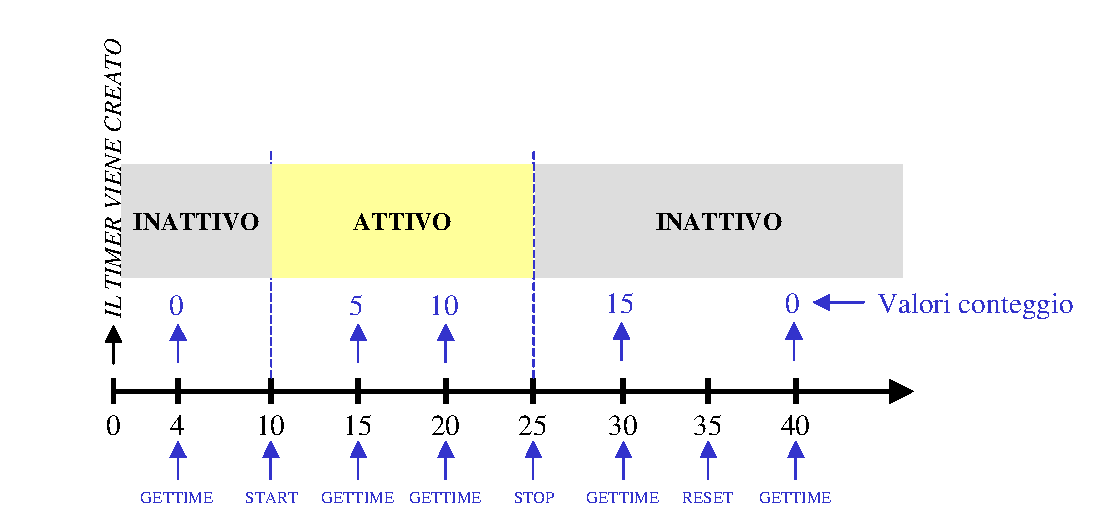
\includegraphics[width=.9\textwidth]{Esercizi/Timer/Timer.eps}
	\caption{Un esempio d'uso del timer nel tempo}
	\label{fig:Timer}	
\end{figure}

Si realizzi una classe \cod{Main} dotata di un metodo \cod{main()} che permetta di effettuare il collaudo della struttura dati realizzata.

Nessuno dei metodi della classe pu� operare con i canali di input/output (per es. \cod{System.out}). L'interfacciamento con l'utente per la lettura e la visualizzazione dei dati sono concessi esclusivamente all'interno della classe \cod{Main}.

\subsubsection*{Suggerimenti}
\begin{itemize}
\item
Le classi standard \cod{java.\-time.\-Local\-Date\-Time} e \cod{java.\-time.\-Duration} implementano il trattamento delle date e delle durate temporali. Consultando la documentazione di queste classi � possibile conoscere i servizi messi da queste a disposizione. Per esempio, la chiamata al metodo \cod{LocalDateTime.now()} restituisce un'istanza della classe \cod{java.\-time.\-Local\-Date\-Time} contenente l'ora corrente del sistema.
\item
Il funzionamento del timer nei casi non espressamente previsti dalle specifiche sia arbitrario.
\end{itemize}
\exercise{Timer Avanzato}
Con riferimento alla classe \cod{Timer} dell'esercizio~\ref{Ex:Timer}, si considerino le seguenti ulteriori specifiche:

\begin{itemize}
\item quando il timer riceve il messaggio START, il conteggio non deve ripartire sempre da 0, ma dal valore correntemente memorizzato;
\item la ricezione di un messaggio START a timer attivo deve essere ininfluente;
\item la ricezione di un messaggio STOP a timer fermo deve essere ininfluente.
\end{itemize}

Modificare, se necessario, l'implementazione del timer per rendere la classe conforme a queste ulteriori specifiche.
\exercise{Votazioni}
Si supponga di voler gestire un exit-poll elettorale. Ad ogni intervistato all'uscita dal seggio si chiede il partito per cui ha votato. In ogni momento bisogna poi essere in grado di dire quanti voti ha ottenuto ciascun partito e qual � la distribuzione dei voti tra i partiti.
Mediante l'uso del costrutto \cod{class} del linguaggio C++, si realizzi una struttura dati adatta all'uopo. Si supponga, per semplicit�, che ogni partito � identificato con un codice intero, e si ignorino i voti bianchi e nulli. Di seguito � riportata la specifica dei metodi pubblici da implementare per la classe \cod{Votazioni}.

\begin{methodslist}

\method{Votazioni}{\emptyset}{\emptyset} {
Costruttore.
}

\method{\~{}Votazioni}{\emptyset}{\emptyset} {
Distruttore.
}

\method{AggiungiVoto}{unsigned int}{unsigned int} {
Aggiunge un voto al partito avente il codice specificato dal parametro di ingresso. Restituisce il numero di voti accumulati fino a quel momento dal partito.
}

\method{Svuota}{\emptyset}{\emptyset} {
Svuota la struttura.
}

\method{GetVotiPartito}{unsigned int}{unsigned int} {
Restituisce il numero di voti ottenuto dal partito avente il codice specificato dal parametro di ingresso.
}

\method{GetNumeroVoti}{\emptyset}{unsigned int} {
Restituisce il numero totale di voti.
}

\method{GetSituazione}{\emptyset}{\emptyset} {
Stampa a video un riepilogo dei voti complessivamente registrati nella struttura.
}

\end{methodslist}

L'unico metodo della classe \cod{Votazioni} che pu� utilizzare lo standard-output (\cod{cout}) � il metodo \cod{GetSituazione()}. Gli altri metodi (pubblici, privati o protetti) non possono fare uso delle funzionalit� di stampa.

Si realizzi una funzione \cod{main()} che permetta di effettuare il collaudo della struttura dati realizzata.

\part{Soluzioni}

\renewcommand{\thechapter}{SL}
\chapter{Soluzioni degli esercizi su liste}
\thesolution{Lista Semplicemente Collegata}%{LinkedList}
Di seguito si riporta il file \cod{Lista.java} contenente la definizione della classe \cod{Lista}. Come richiesto dalla traccia, la lista � semplicemente collegata e le sue celle sono rappresentate dalla classe \cod{Record}, definita all'interno della classe \cod{Lista}. Grazie al modificatore di accesso \cod{private}, la classe \cod{Record} resta invisibile agli utenti della classe contenitore. Dall'interfaccia della classe \cod{Lista} non traspare la sua natura di lista semplicemente collegata. I dettagli implementativi restano pertanto nascosti, nel rispetto del principio dell'\emph{information hiding}.

In questa implementazione il costruttore dovrebbe avere il compito di inizializzare le variabili-membro della classe, che in questo caso sono \cod{first} e \cod{numEl}. L'inizializzazione dovrebbe consistere nelle seguenti due istruzioni:

\begin{codequote}
	first = null;
	numEl = 0;
\end{codequote}

In assenza di queste due linee, per�, le specifiche del linguaggio Java indicano che \cod{first} viene inizializzato a \cod{null} (default per gli oggetti) e \cod{numEl} a \cod{0} (default per gli interi). Tale inizializzazione � pertanto superflua e il costruttore pu� rimanere vuoto.

\inputmodule{Lista.java}{Esercizi/LinkedList/Lista.java}

Il modulo \cod{Main.java}, di seguito riportato, consente di effettuare il testing di tutte le funzionalit� disponibili nella classe \cod{Lista}. L'interfacciamento con l'utente � testuale e basato su console.

\inputmodule{Main.java}{Esercizi/LinkedList/Main.java}
\thesolution{Somma Elementi}

Il metodo effettua una visita completa della lista. Ad ogni iterazione somma ad un accumulatore il valore della cella correntemente visitata.

\inputprogram{Esercizi/SommaElementi/SommaElementi.java}
\thesolution{Coda Pari}
Per valutare se l'elemento di coda � pari � possibile adottare un approccio iterativo che, a partire dall'elemento di testa, ricerchi l'ultimo elemento e ne restituisca il valore.

\inputprogram{Esercizi/CodaPari/CodaPari.java}

L'esercizio pu� essere anche risolto secondo un approccio ricorsivo, cos� come riportato di seguito.

\inputprogram{Esercizi/CodaPari/CodaPari_ric.java}
\thesolution{Min e Max}
La ricerca del minimo e del massimo possono essere condotte secondo un approccio iterativo. Nel listato che segue, si assume inizialmente che il minimo ed il massimo siano entrambi rappresentati dall'elemento di testa (linee 3 e 4). Successivamente si scandiscono in sequenza gli elementi della lista. Ogni volta che viene individuato un elemento minore del minimo corrente (linea 8), il minimo corrente viene aggiornato (linea 9). Analogo discorso vale per il massimo (linee 10 e 11).

\enablelstnum
\inputprogram{Esercizi/MinMax/MinMax.cpp}
\thesolution{Lista Statica}

La soluzione prevede l'uso di un vettore per ospitare gli elementi della lista. La dimensione del vettore � specificata dalla costante privata \cod{MAXEL} definita nella classe \cod{Lista} e vincola il numero massimo di elementi che possono essere inseriti.

\inputprogram{Esercizi/ListaStatica/ListaStatica.java}
\thesolution{\`E Ordinata}
\inputprogram{Esercizi/EOrdinata/EOrdinata.java}
\thesolution{Elimina Tutti}
Ipotizzando che l'elemento da eliminare sia \cod{0}, il metodo \cod{eliminaTutti()} modifica il vettore degli elementi come mostrato in \figurename~\ref{fig:EliminaTutti}.

\begin{figure}
  \center
	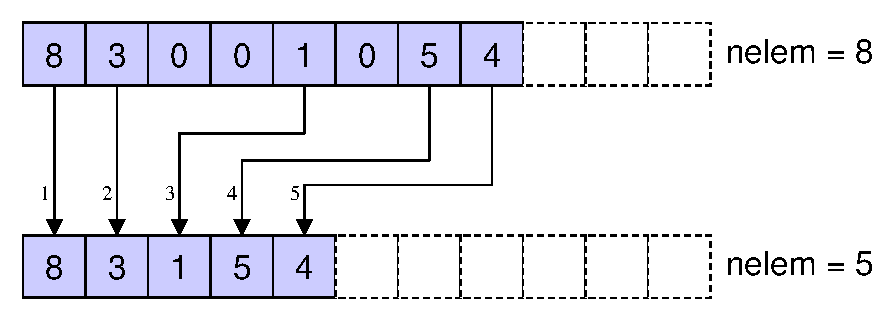
\includegraphics[width=.75\textwidth]{Esercizi/EliminaTutti/EliminaTutti.eps}
	\caption{Eliminazione degli elementi con valore \cod{0} dal vettore}
	\label{fig:EliminaTutti}
\end{figure}

Per ottenere l'effetto desiderato � sufficiente scandire in sequenza gli elementi del vettore originario (in alto nella figura). Ad ogni passo, se l'elemento puntato � diverso dall'elemento da eliminare, lo si ricopia nel vettore in basso; in caso contrario non si effettua alcuna operazione e si passa ad analizzare l'elemento successivo. Alla fine della scansione il vettore in basso risulter� composto dai soli elementi del vettore originario diversi da quello da eliminare.

\`E facile convincersi del fatto che, per realizzare l'operazione appena descritta, non sia necessario utilizzare due distinti vettori, ma tutto il procedimento pu� essere svolto su un unico vettore. La copia di un elemento diviene in questo caso uno spostamento nell'ambito dello stesso vettore, senza che la sovrascrittura della locazione di destinazione rappresenti un problema. Allo scopo � sufficiente utilizzare due indici \cod{i} e \cod{j}:
\begin{itemize}
\item{\cod{i}} va da \cod{0} a $\cod{nelem-1}$, scandendo in sequenza tutti gli elementi del vettore originario;
\item{\cod{j}} avanza ogni qual volta un elemento viene ``ricopiato'', e pertanto rappresenta il riempimento corrente del vettore ``ripulito''.
\end{itemize}

Di seguito si riporta il codice del metodo \cod{eliminaTutti()}.

\bigskip
\inputprogram{Esercizi/EliminaTutti/EliminaTutti.java}
\bigskip
\thesolution{Elimina Ultimi}
Il metodo \cod{lasciaPrimi()} richiede di eliminare gli ``elementi di coda'' della lista, preservandone i primi \cod{n}. Bisogna dapprima considerare i seguenti casi degeneri:

\begin{itemize}
\item il numero di elementi da conservare � maggiore del numero di elementi presenti nella lista: nessun elemento va eliminato (righe 2--3);
\item il numero degli elementi da conservare � pari a zero: tutti gli elementi vanno eliminati (righe 6--11).
\end{itemize}

Negli altri casi, bisogna dapprima scorrere attraverso le prime \cod{n} posizioni della lista (righe 17--18); i restanti elementi dovranno essere scollegati dalla lista (riga 20). L'implementazione risultante � la seguente.

\bigskip
\enablelstnum
\inputprogram{Esercizi/EliminaUltimi/LasciaPrimi.java}
\bigskip

Il metodo \cod{eliminaUltimi()} deve eliminare gli ultimi \cod{n} elementi. Esso non differisce nella sostanza dal precedente metodo, e pu� essere pertanto implementato nei termini di quest'ultimo.

\bigskip
\inputprogram{Esercizi/EliminaUltimi/EliminaUltimi.java}
\bigskip
\thesolution{Somma Coda}
L'approccio in generale pi� efficiente per risolvere questo problema consiste nel tenere memoria in un membro privato della lista del valore della coda. Tale valore deve essere costantemente aggiornato, a cura di tutti i metodi che possono potenzialmente alterarlo: inserimento, eliminazione, svuotamento, ecc. Si noti che lo stesso metodo \cod{SommaCoda()} finisce per alterare il valore della coda. Di seguito si mostrano le implementazioni dei metodi \cod{Inserisci()} e \cod{SommaCoda()}, nelle ipotesi che la lista sia dotata di una variabile-membro privata definita come segue:

\begin{codequote}
  class Lista {
  private:
    ...
    TElem valoreCoda;
    ...
  };
\end{codequote}

\bigskip
\inputprogram{Esercizi/SommaCoda/SommaCoda.cpp}
\thesolution{Sposta Testa in Coda}
Per svolgere l'operazione si fa uso di un metodo di supporto \cod{getPuntCoda()} deputato a restituire il puntatore all'elemento di coda della lista, se esistemte. Si noti che nessun nuovo elemento viene creato (\cod{new}), ma l'operazione � effettuata esclusivamente mediante ricollocazione di puntatori, preservando le caratteristiche di efficienza della soluzione.

\bigskip
\inputprogram{Esercizi/SpostaTestaInCoda/SpostaTestaInCoda.java}
\thesolution{Elimina Pari e Dispari}
\inputprogram{Esercizi/EliminaPariDispari/EliminaPariDispari.java}
\thesolution{Lista Doppiamente Collegata}
\inputmodule{Lista.java}{Esercizi/ListaDoppiamenteCollegata/Lista.java}
\inputmodule{Main.java}{Esercizi/ListaDoppiamenteCollegata/Main.java}
\thesolution{Ribalta}
L'approccio in generale pi� efficiente per ribaltare la lista consiste nel modificare la configurazione di tutti i puntatori contenuti nella struttura, senza pertanto effettuare spostamenti fisici di elementi. Di seguito si forniscono due soluzioni, la prima basata su un metodo iterativo, la seconda su uno ricorsivo.

\begin{figure}
  \begin{center}
    \begin{minipage}{.8\textwidth}
      \subfigure[Lista originale]{
        \centering
        \label{fig:Originale}
        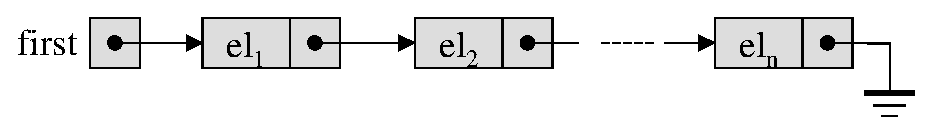
\includegraphics[width=.9\textwidth]{Esercizi/Ribalta/Originale.eps}
      }%
    \end{minipage}
    \hfill
    \begin{minipage}{.6\textwidth}
      \subfigure[Prima dell'i-esima iterazione]{
        \centering
        \label{fig:PrimaDelWhile}
        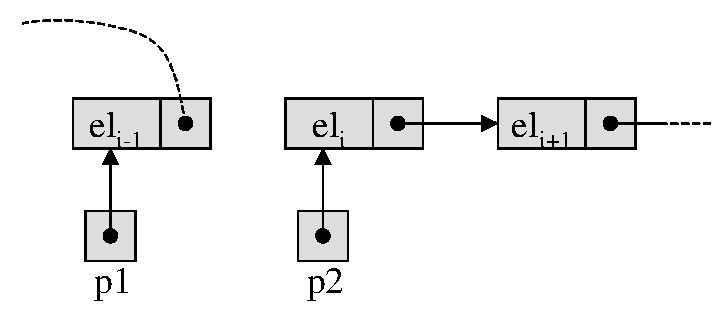
\includegraphics[width=.9\textwidth]{Esercizi/Ribalta/PrimaDelWhile.eps}
      }%
    \end{minipage}
    \hfill
    \begin{minipage}{.6\textwidth}
      \subfigure[Dopo l'i-esima iterazione]{
        \centering
        \label{fig:DopoIlWhile}
        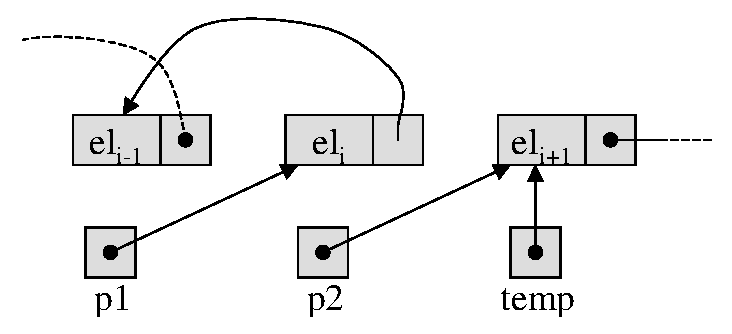
\includegraphics[width=.9\textwidth]{Esercizi/Ribalta/DopoIlWhile.eps}
    }
    \end{minipage}
    \hfill
    \begin{minipage}{.8\textwidth}
      \subfigure[Lista ribaltata]{
        \centering
        \label{fig:Ribaltata}
        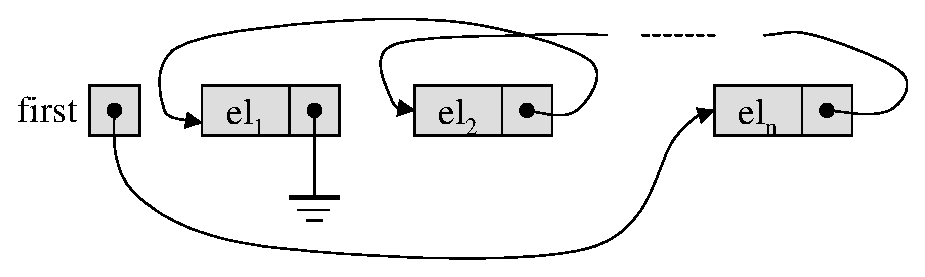
\includegraphics[width=.9\textwidth]{Esercizi/Ribalta/Ribaltata.eps}
    }
    \end{minipage}
  \end{center}
  \caption{Il processo logico di ribaltamento di una lista}
  \label{fig:Ribaltamento}
\end{figure}

\subsubsection*{Approccio iterativo}
Si consideri la \figurename~\ref{fig:Originale}, in cui � riportata la lista di partenza. Per ottenerne il ribaltamento � sufficiente che il campo \cod{succ} del primo elemento (che punta ad $el_2$) passi a puntare a 0, che il campo \cod{succ} del secondo elemento (che punta ad $el_3$) passi a puntare al primo, che il campo \cod{succ} del terzo elemento (che punta ad $el_4$) passi a puntare al secondo\ldots\ e cos� via. Infine, il puntatore \cod{first} (che punta ad $el_1$) dovr� puntare all'elemento $el_n$. Questo procedimento pu� essere svolto servendosi di due puntatori che iniziano a scorrere la lista nell'unica direzione concessa, puntando di volta in volta a due elementi consecutivi e spostandosi in avanti di un elemento alla volta. Ad ogni passo dell'iterazione lo scambio pu� essere effettuato servendosi di un terzo puntatore temporaneo (vedi Figure~\ref{fig:PrimaDelWhile} e~\ref{fig:DopoIlWhile}). Lo stato finale della lista al termine dell'iterazione � riportato in \figurename~\ref{fig:Ribaltata}.

%\begin{figure}
%  \begin{center}
%    \begin{minipage}{.8\textwidth}
%      \subfigure[prima dell'i-esima iterazione]{
%        \centering
%        \label{fig:PrimaDelWhile}
%        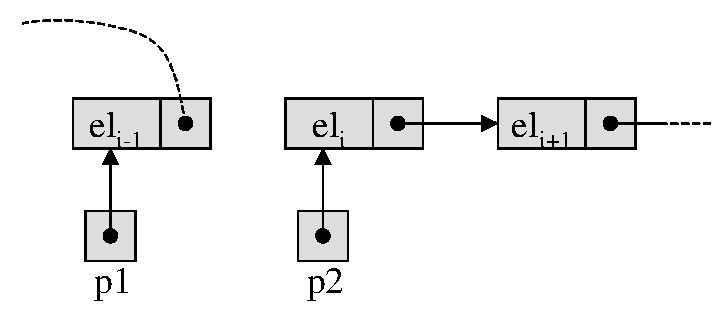
\includegraphics[width=.9\textwidth]{Esercizi/Ribalta/PrimaDelWhile.eps}
%      }%
%    \end{minipage}
%    \hfill
%    \begin{minipage}{.8\textwidth}
%      \subfigure[dopo l'i-esima iterazione]{
%        \centering
%        \label{fig:DopoIlWhile}
%        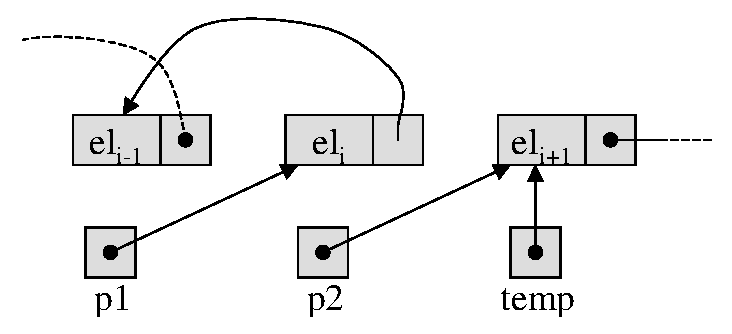
\includegraphics[width=.9\textwidth]{Esercizi/Ribalta/DopoIlWhile.eps}
%    }
%    \end{minipage}
%  \end{center}
%  \caption{Effetto dell'i-esima iterazione}
%  \label{fig:iesimaiterazione}
%\end{figure}

\bigskip
\inputprogram{Esercizi/Ribalta/Ribalta_iterativo.cpp}

\subsubsection*{Approccio ricorsivo}
Il ribaltamento della lista pu� essere approcciato come un problema ricorsivo. Infatti, avendo una lista, la sua versione ribaltata si ottiene isolando il primo elemento, ribaltando la restante parte della lista, e posponendo a questa l'elemento isolato. Il problema del ribaltamento di una lista si riconduce dunque al ribaltamento di una seconda lista costituita da un elemento in meno. Di questo passo ci si trover� a ribaltare una lista costituita da un unico elemento, la cui versione ribaltata � uguale a s� stessa. Durante il processo di ribaltamento bisogna anche prestare attenzione a redirigere correttamente la testa della (sotto)lista di volta in volta considerata. A questo proposito, il metodo ricorsivo \cod{\_Ribalta()} riceve in ingresso il puntatore alla testa della lista da ribaltare e restituisce la testa della lista ribaltata.

\bigskip
\inputprogram{Esercizi/Ribalta/Ribalta_ricorsivo.cpp}

\renewcommand{\thechapter}{SA}
\chapter{Soluzioni degli esercizi su alberi binari}
\thesolution{Albero Binario}
\inputmodule{AlberoBinario.java}{Esercizi/AlberoBinario/AlberoBinario.java}
\inputmodule{main.java}{Esercizi/AlberoBinario/main.java}
\thesolution{Numero Elementi}
La tecnica pi� semplice per effettuare il conteggio del numero di elementi contenuti in un albero, consiste nel definire un membro privato di tipo intero non negativo atto a memorizzare tale valore. Il valore del membro viene alterato da tutti i metodi della struttura che modificano il numero di nodi presenti in essa (inserimento, eliminazione, svuotamento, ecc.).

Qui si mostrer� un approccio differente, in generale meno efficiente, consistente in un metodo ricorsivo che calcola il numero di elementi mediante una visita completa dell'albero.

\bigskip
\inputprogram{Esercizi/NumeroElementi/NumElem.java}
\thesolution{Occorrenze}
\inputprogram{Esercizi/Occorrenze/Occorrenze.java}
\thesolution{Occorrenza Massima}
Per risolvere il problema bisogna apportare alcune modifiche alla classe \cod{Al\-be\-ro\-Bi\-na\-rio} dell'esercizio �\ref{Ex:Albero Binario}. In particolare va modificato il costruttore, perch� acquisisca il valore \cod{occMax}. Inoltre, il metodo ricorsivo \cod{\_ag\-giun\-gi\-E\-lem()} ora deve restituire non pi� solo il valore del nodo creato, ma anche il valore \cod{boolean} che indica l'esito dell'inserimento. \`E pertanto opportuno confezionare una classe, che chiameremo \cod{Da\-ti\-Ag\-giun\-ta} con visibilit� privata, che convoglier� fuori dal metodo ricorsivo i due valori richiesti. Le modifiche descritte sono mostrate nel listato seguente.

\inputprogram{Esercizi/MaxOcc/SintesiModifiche.java}

Particolare attenzione merita il metodo \cod{\_ag\-giun\-gi\-E\-lem()}, che si occupa dell'inserimento nell'albero
dell'elemento specificato dal parametro di ingresso, nel rispetto del vincolo delle occorrenze massime. Esso si basa sulla propriet� secondo la quale, durante l'inserimento di un elemento in un albero binario ordinato, bisogna necessariamente attraversare tutti gli eventuali altri nodi contenenti lo stesso valore da inserire. \`E possibile dunque discendere attraverso l'albero in cerca della posizione in cui aggiungere l'elemento e, contemporaneamente, tenere il conteggio dell'occorrenza delle eventuali repliche, interrompendo prematuramente l'inserimento in caso di raggiungimento del numero massimo di occorrenze.

L'implementazione dei metodi \cod{ag\-giun\-gi\-E\-lem()} (pubblico non ricorsivo) e \cod{\_ag\-giun\-gi\-E\-lem} (privato ricorsivo) � riportata di seguito.

\inputprogram{Esercizi/MaxOcc/MaxOcc.java}
\thesolution{Profondit� Limitata}
L'interfaccia della classe \cod{AlberoBinario} da realizzare � mostrata di seguito, con enfasi sulle modifiche da applicare alla versione della classe presentata in �\ref{Ex:Albero Binario}.

\begin{codequote}
  class AlberoBinario {
  private:
    ...
    const unsigned int maxDepth;
    ...
  public:
    AlberoBinario(unsigned int _maxDepth);
    ...
    bool Inserisci(const TElem& el);
    ...
  };
\end{codequote}

\inputprogram{Esercizi/MaxProf/MaxProf.cpp}
\thesolution{Somma}
\inputprogram{Esercizi/Somma/Somma.cpp}
\thesolution{Sostituisci}
\inputprogram{Esercizi/Sostituisci/Sostituisci.cpp}
\thesolution{Conta Min e Max}
Il conteggio degli elementi compresi entro un certo intervallo pu� essere svolto mediante una visita dell'albero. Data la propriet� di ordinamento dell'albero, non � peraltro necessario visitare completamente la struttura. Si consideri per esempio il caso in cui si debbano conteggiare gli elementi compresi nell'intervallo $[10,20]$. In occasione della visita di un ipotetico elemento pari a $5$, � inutile procedere verso il sottoalbero sinistro di tale elemento, che non ha possibilit� di fornire un contributo al conteggio in corso.

\inputprogram{Esercizi/ContaMinMax/ContaMinMax.java}
\thesolution{Profondit� Maggiore di Due}
Si noti che il metodo riportato di seguito non � ricorsivo, n� richiama alcun altro metodo.

\bigskip
\inputprogram{Esercizi/ProfonditaMaggioreDiDue/ProfonditaMaggioreDiDue.cpp}
\thesolution{Profondita Maggiore Di}
\inputprogram{Esercizi/ProfonditaMaggioreDi/ProfonditaMaggioreDi.java}
\thesolution{Profondit� Massima}
Il metodo \cod{profondita()} deve restituire un'informazione strutturata:
\begin{itemize}
\item la profondit� massima dell'elemento eventualmente trovato;
\item il tipo del nodo eventualmente trovato, foglia o non-foglia.
\end{itemize}

Per restituire questa informazione viene utilizzata un'apposita classe denominata \cod{InfoProf}. Laddove l'elemento non venisse trovato, il metodo restituirebbe un riferimento \cod{null}.

\inputprogram{Esercizi/ProfonditaMax/ProfonditaMax.java}
\thesolution{Somma Livello}
\inputprogram{Esercizi/SommaLivello/SommaLivello.java}
\thesolution{Eliminazione Foglia}
\inputprogram{Esercizi/EliminaFoglia/EliminaFoglia.java}
\thesolution{Eliminazione Foglie}
\inputprogram{Esercizi/EliminaFoglie/AlberoBinario.cpp}
\thesolution{Cerca Foglia}
I metodi \cod{cercaFoglia()} e \cod{cercaNodo()} devono restituire un'informazione strutturata, costituita da due valori logici. Come di consueto, saranno utilizzate allo scopo delle classi appositamente definite. In questo caso si � scelto di realizzare questa classi come \emph{classi immutabili}. Ci� significa che il valore di ogni loro istanza viene definito all'atto della creazione e non pu� essere variato per tutto il ciclo di vita. Per esempio, il costruttore della classe \cod{RisultatoRicercaFoglia} � definito come segue:

\enablelstnum
\begin{codequote}
		public RisultatoRicercaFoglia(boolean trovato,
		        boolean foglia) {
			this.trovato = trovato;
			this.foglia = foglia;
		}
\end{codequote}
\disablelstnum

Le righe $1$ e $2$ contengono i parametri di ingresso, utili ad assegnare il valore delle omonime variabili private contenute nella classe. L'omonimia non crea alcun problema poich�, nello scope in cui sono visibili sia le variabili private che i parametri locali (righe $3$ e $4$), viene risolta utilizzando il prefisso \cod{this}. Laddove � presente \cod{this} ci si sta riferendo alla variabile membro privata. Laddove \cod{this} non � presente, si fa invece riferimento al parametro locale.

Di seguito � riportata l'implementazione dei metodi pubblici e privati utili a rispondere alla traccia.

\inputprogram{Esercizi/CercaFoglia/CercaFoglia.java}
\thesolution{Operatore di Confronto}
Il metodo \cod{equals()} deve innanzitutto verificare che l'istanza di oggetto passata in ingresso sia della classe \cod{AlberoBinario}. A questo scopo si utilizza l'operatore del linguaggio \cod{instanceof}, che restituisce un valore booleano. Se questo operatore restituisce il valore \cod{false}, il metodo termina prematuramente con il valore \cod{false}. Altrimenti si procede alla verifica sull'uguaglianza strutturale tra i due alberi da confrontare.

Si noti come la variabile \cod{alb} del metodo \cod{equals()} rappresenti un ulteriore riferimento all'oggetto \cod{obj}: bench� i due riferimenti siano identici (puntino cio� alla medesima locazione di memoria), il loro tipo � differente e \cod{alb} pu� essere utilizzato come parametro attuale nella chiamata del metodo ricorsivo \cod{\_equals()}.

\inputprogram{Esercizi/OperatoreConfronto/OperatoreConfronto.java}
\thesolution{Conta Nodi non Foglia}
\inputprogram{Esercizi/ContaNodiNonFoglia/ContaNodiNonFoglia.java}
\thesolution{Conta Nodi}
La restituzione dei tre valori richiesti da parte del metodo \cod{contaNodi()} avviene mediante l'istanza di una classe \cod{ConteggioNodi}, appositamente definita. La classe implementa anche un metodo di supporto utile ad effettuare la somma tra due istanze della classe medesima.

\inputprogram{Esercizi/ContaNodi/ContaNodi.java}
\thesolution{Conta Nodi Sottoalbero}
Il problema posto pu� essere scomposto in due sottoproblemi:
\begin{itemize}
  \item individuare la radice del sottoalbero di cui contare i nodi;
  \item contare i nodi del sottoalbero individuato.
\end{itemize}
Solo la prima delle due operazioni suddette dipende da quale dei due metodi viene invocato, a differenza della seconda che resta inalterata. Questa considerazione suggerisce di aggiungere alla classe \cod{AlberoBinario} i seguenti metodi:

\begin{codequote}
  class AlberoBinario {
  private:
    ...
    
    unsigned int _ContaNodi(const PNodo& n) const;
    PNodo _CercaOccorrenzaMin(const PNodo& n,
      const TElem& el) const;
    PNodo _CercaOccorrenzaMax(const PNodo& n,
      const TElem& el) const;
   public:
    ...

    unsigned int ContaNodiSottoalb_Min(const TElem& el) const;
    unsigned int ContaNodiSottoalb_Max(const TElem& el) const;
  };
\end{codequote}

Il metodo \cod{\_ContaNodi()} restituisce il numero di nodi di un sottoalbero di cui sia fornita la radice. Il metodo \cod{\_CercaOccorrenzaMin()} restituisce il puntatore al nodo avente valore specificato e posizionato pi� in alto (livello minimo) all'interno di un albero di cui si fornisce la radice. Analogo comportamento ha il metodo \cod{\_CercaOccorrenzaMax()}. I due metodi pubblici svolgono le operazioni richieste basandosi sui metodi privati mostrati. \cod{\_CercaOccorrenzaMin()}, ad esempio, invoca il metodo ricorsivo \cod{\_Cerca\-Oc\-cor\-ren\-za\-Min()} perch� individui la radice del sottoalbero; su tale radice invoca poi il metodo \cod{\_ContaNodi()}.

Di seguito si riportano le implementazioni dei cinque metodi dichiarati.

\inputprogram{Esercizi/ContaNodiSottoalbero/ContaNodiSottoalbero.cpp}
\thesolution{SommaMinMax}
\inputprogram{Esercizi/SommaMinMax/SommaMinMax.java}

\renewcommand{\thechapter}{SP}
\chapter{Soluzioni degli esercizi su pile}
\thesolution{Push Greater}
\inputprogram{Esercizi/PushGreater/Pila.cpp}
\thesolution{Push If}
Nella parte privata della classe sono dichiarati i seguenti membri:

\begin{codequote}
  class Pila {
  private:
    ...
    const unsigned int _maxpush;
    unsigned int _currpush;
    void _Push(const TElem& e);
    ...
  };  
\end{codequote}

La variabile membro \cod{\_maxpush} tiene memoria di qual � il numero di inserimenti massimi consecutivi ammessi; il suo valore � inizializzato dal costruttore al valore del parametro di ingresso e mai pi� variato durante il ciclo di vita delle istanze della classe. La variabile membro \cod{\_currpush} tiene memoria del numero di inserimenti consecutivi correntemente effettuati. Ogni chiamata al metodo \cod{Push()} deve verificare che questo parametro non ecceda il valore massimo consentito. Il metodo privato \cod{\_Push()} � implementato come una classica \cod{Push()}.

Di seguito si riporta l'implementazione dei metodi richiesti dalla traccia.

\inputprogram{Esercizi/PushIf/Pila.cpp}

\renewcommand{\thechapter}{SC}
\chapter{Soluzioni degli esercizi su code}
\thesolution{Coda}
\inputmodule{Coda.java}{Esercizi/Coda/Coda.java}
\inputmodule{Main.java}{Esercizi/Coda/Main.java}
\thesolution{Coda con Perdite}
\inputprogram{Esercizi/CodaConPerdite/CodaConPerdite.cpp}
\thesolution{Coda a Priorit�}
Si vuole una coda in cui gli elementi possano essere liberamente accodati e siano connotati da uno tra due possibili livelli di priorit�. Il prelievo di un elemento dalla coda dovr� rispettare, in primis, il livello di priorit� e, nell'ambito degli elementi aventi la stessa priorit�, la disciplina \emph{first-in-first-out} (FIFO) di una coda.

La traccia specifica esclusivamente il comportamento ``esteriore'' della struttura dati, senza definire alcun dettaglio di natura implementativa. Per ottenere una struttura avente il comportamento specificato � possibile seguire diverse strade. Di seguito sono riportate alcune possibilit�.

\subsection*{Approccio 1}
La coda a priorit� pu� essere immaginata formata da una sequenza di elementi costituita a sua volta da due sotto-sequenze (\seename\ \figurename~\ref{fig:SottoSequenze}):
\begin{itemize}
\item una prima sotto-sequenza, che parte dalla testa, che comprende gli elementi a priorit� alta;
\item una successiva sotto-sequenza, che si estende fino alla coda, che comprende gli elementi a priorit� bassa.
\end{itemize}
Una o entrambe queste sotto-sequenze possono in generale essere vuote.

Dal momento che le operazioni di prelievo (\cod{Pop()}) e di inserimento a bassa priorit� (\cod{PushLow()}) corrispondono in questo caso alle normali operazioni usate nel caso di una classica coda, l'unica operazione nuova da implementare consiste nell'inserimento in coda di un elemento a priorit� alta (\cod{PushHigh()}). Tale operazione prevede l'aggiunta di un elemento ``in coda'' agli elementi a priorit� alta. In quest'ottica risulta utile definire un puntatore \cod{h} aggiuntivo posizionato sull'ultimo degli elementi a priorit� alta.
Tale nuovo puntatore punter� alla coda degli elementi ad alta priorit�, oppure varr� zero in caso di assenza di tali elementi.

\begin{figure}
  \center
	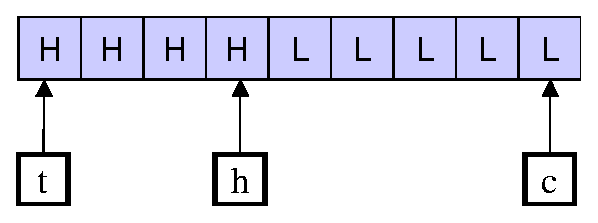
\includegraphics[width=.5\textwidth]{Esercizi/CodaAPriorita/2.eps}
	\caption{Una sequenza di elementi formata da due sotto-sequenze consecutive}
	\label{fig:SottoSequenze}
\end{figure}

\inputmodule{PriorityQueue.h}{Esercizi/CodaAPriorita/1/PriorityQueue.h}
\inputmodule{PriorityQueue.cpp}{Esercizi/CodaAPriorita/1/PriorityQueue.cpp}

\subsection*{Approccio 2}
La coda a priorit� pu� essere immaginata composta di due classiche code affiancate (\seename\ \figurename~\ref{fig:CodeAffiancate}), ciascuna destinata a contenere gli elementi di una singola classe. Il metodo \cod{PushLow()} accoda nella coda a bassa priorit�. Il metodo \cod{PushHigh()}, viceversa, in quella ad alta priorit�. Il metodo \cod{Pop()} restituisce l'elemento di testa nella coda ad alta priorit�, se esiste; in caso contrario restituisce l'elemento di testa nella coda a bassa priorit�.

Servendosi del meccanismo dell'aggregazione stretta tra classi, le due code affiancate risultano istanze della classe \cod{Coda} (\cfr{Ex:Coda}). Definendo tali istanze come membri privati della classe \cod{PriorityQueue} esse non risulteranno visibili dall'esterno della struttura (\emph{information hiding}), la quale continuer� ad apparire ai suoi utenti come una singola coda dotata dei meccanismi di priorit� richiesti.

\begin{figure}
  \center
	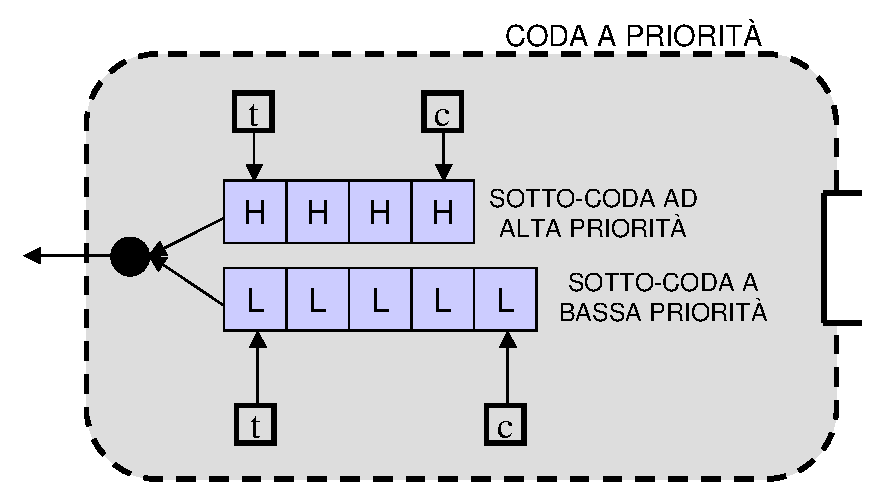
\includegraphics[width=.7\textwidth]{Esercizi/CodaAPriorita/4.eps}
	\caption{Coda a priorit� formata da due classiche code affiancate}
	\label{fig:CodeAffiancate}
\end{figure}

\inputprogram{Esercizi/CodaAPriorita/2/PriorityQueue.h}
\inputprogram{Esercizi/CodaAPriorita/2/PriorityQueue.cpp}

\subsection*{Approccio 3}
La coda a priorit� pu� essere una normale coda in cui i record, disposti secondo l'ordine di inserimento, vengono etichettati con la loro priorit�\footnote{Questo � possibile previa definizione di un'opportuna \cod{struct} che contenga un \cod{TElem} ed un \cod{bool} indicante la relativa priorit�.} (\seename\ \figurename~\ref{fig:ElementiEtichettati}). In questo caso sia il metodo \cod{PushHigh()} che il metodo \cod{PushLow()}, previa opportuna etichettatura, effettuano un'aggiunta in coda. \`E il metodo \cod{Pop()} in questo caso a prendersi carico della restituzione del ``giusto'' elemento. Tale operazione viene effettuata scorrendo tutta la struttura alla ricerca del primo elemento ad alta priorit� e restituendolo dopo averlo eliminato dalla coda. In assenza di un elemento ad alta priorit� viene restituito l'eventuale elemento di testa.

\begin{figure}
  \center
	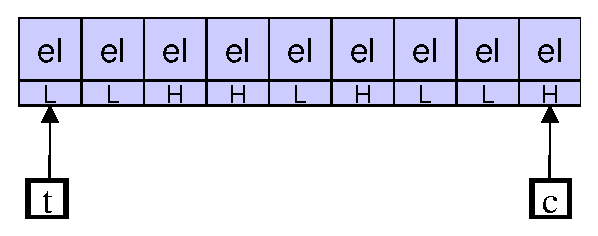
\includegraphics[width=.5\textwidth]{Esercizi/CodaAPriorita/3.eps}
	\caption{Sequenza di elementi ``etichettati''}
	\label{fig:ElementiEtichettati}
\end{figure}

Tale implementazione, pur prestandosi a diverse ottimizzazioni, non risulta particolarmente efficiente, richiedendo un ciclo di ricerca per ogni operazione \cod{Pop()} effettuata. La sua implementazione non � qui riportata.
\thesolution{PopMinMax}
\inputprogram{Esercizi/PopMax/PopMax.cpp}

\renewcommand{\thechapter}{SX}
\chapter{Soluzioni degli altri esercizi}
\thesolution{Accumulatore}%{Accumulatore}
\inputmodule{Accumulatore.java}{Esercizi/Accumulatore/Accumulatore.java}
\inputmodule{Main.java}{Esercizi/Accumulatore/Main.java}
\thesolution{Cifratore}
\inputmodule{Cifratore.java}{Esercizi/Cifratore/Cifratore.java}
\inputmodule{Main.java}{Esercizi/Cifratore/Main.java}
\thesolution{Lista Della Spesa}
L'attributo \emph{nome} della classe \cod{Articolo} � immutabile: il suo valore � pertanto inizializzato contestualmente alla costruzione e mai pi� modificato per tutto il ciclo di vita della relativa istanza. La clausola \cod{final} serve proprio a forzare tali controlli da parte del compilatore.
\inputmodule{Articolo.java}{Esercizi/ListaDellaSpesa/Articolo.java}
\inputmodule{ListaDellaSpesa.java}{Esercizi/ListaDellaSpesa/ListaDellaSpesa.java}
\inputmodule{Main.java}{Esercizi/ListaDellaSpesa/Main.java}
\thesolution{Predittore di Temperatura}
Il metodo \cod{estimateTemp()} deve effettuare un'estrapolazione lineare della temperatura basandosi sui dati delle ultime due letture comunicate. La formula da utilizzare � la seguente:

%                  T2-T1
%            ET = ------- (t-t1) + T1;
%                  t2-t1

$$\hat{T} = \frac{T_2-T_1}{t_2-t_1}(t-t_1)+T_1;$$
                  
dove $\hat{T}$ � la stima della temperatura all'istante $t$; $T_1$, $T_2$, $t_1$ e $t_2$ sono le ultime due letture della temperatura ed i relativi due istanti di lettura, rispettivamente.

\bigskip
\begin{footnotesize}
N.B.: Variando l'implementazione del metodo \cod{estimateTemp()} si possono operare stime pi� accurate della temperatura; si potrebbe per esempio pensare di operare estrapolazioni di ordine superiore al primo. Per giunta ci�, non alterando l'interfaccia della classe, non comprometterebbe in alcun modo l'integrazione con i moduli utenti del predittore gi� realizzati.
\end{footnotesize}

\bigskip
\inputmodule{TempPredictor.java}{Esercizi/PredittoreTemperatura/TempPredictor.java}
\inputmodule{Main.java}{Esercizi/PredittoreTemperatura/Main.java}
\thesolution{Contenitore}
\inputprogram{Esercizi/Contenitore/Contenitore.cpp}
\thesolution{Lista Prenotazioni}
\inputprogram{Esercizi/ListaPrenotazioni/ListaPrenotazioni.cpp}
\thesolution{Classifica}
\inputmodule{Squadra.java}{Esercizi/Classifica/Squadra.java}
\inputmodule{Classifica.java}{Esercizi/Classifica/Classifica.java}
\inputmodule{Main.java}{Esercizi/Classifica/Main.java}
\thesolution{Agenzia Matrimoniale}
\inputmodule{Persona.java}{Esercizi/AgenziaMatrimoniale/Persona.java}
\inputmodule{AgenziaMatrimoniale.java}{Esercizi/AgenziaMatrimoniale/AgenziaMatrimoniale.java}
\inputmodule{Main.java}{Esercizi/AgenziaMatrimoniale/Main.java}
\thesolution{Parco Pattini}
La struttura dati pu� essere realizzata come una lista dinamica semplicemente collegata in cui ogni elemento rappresenta lo stato di tutti i pattini di una data taglia. La generica cella della struttura contiene dunque:

\begin{itemize}
\item taglia dei pattini;
\item numero totale di pattini della taglia data;
\item numero totale di pattini disponibili della taglia data.
\end{itemize}
    
A titolo esemplificativo si immagini che il parco pattini disponga di un paio di pattini della taglia 44, di un paio della taglia 43 e di due paia della taglia 42. Se uno delle due paia di pattini della taglia 42 risulta fittato, lo stato della struttura � mostrato in \figurename~\ref{fig:Pattini}.
  
\begin{figure}
  \center
	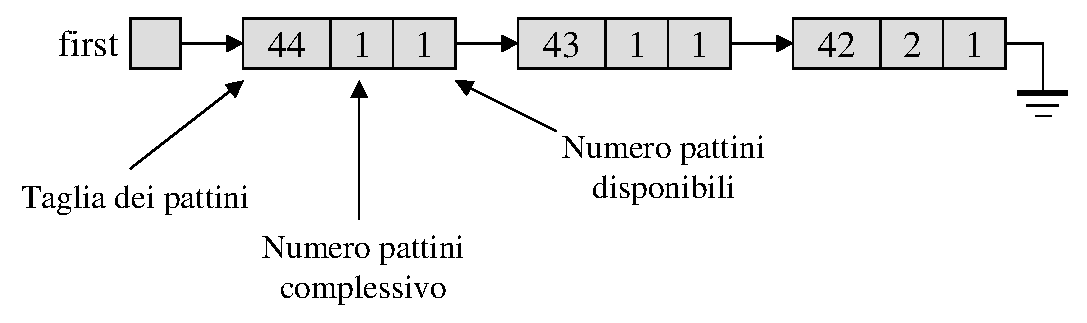
\includegraphics[width=.8\textwidth]{Esercizi/ParcoPattini/pattini.eps}
	\caption{La struttura che implementa il parco pattini.}
	\label{fig:Pattini}
\end{figure}

Si noti come la struttura ammetta una gestione di tipo tabellare, dal momento che la taglia dei pattini risulta essere unica per ogni cella, e quindi assimilabile ad una chiave.

Di seguito si riporta il listato.

\bigskip
\inputmodule{StatoTaglia.java}{Esercizi/ParcoPattini/StatoTaglia.java}
\inputmodule{ParcoPattini.java}{Esercizi/ParcoPattini/ParcoPattini.java}
\inputmodule{Main.java}{Esercizi/ParcoPattini/Main.java}
\thesolution{Timer}
\inputmodule{Timer.java}{Esercizi/Timer/Timer.java}
\inputmodule{Main.java}{Esercizi/Timer/Main.java}
\thesolution{Timer Avanzato}
Il primo dei requisiti aggiuntivi imposti dalla traccia suggerisce intuitivamente che il timer � una sorta di accumulatore che tiene memoria della durata complessiva degli intervalli di tempo cronometrati fino ad un certo istante. Infatti l'esecuzione di un nuovo conteggio fornisce un contributo che va a sommarsi a tutti gli eventuali contributi precedenti. 

Ai fini dello svolgimento di questo esercizio, il valore corrente del cronometro pu� essere pertanto considerato come la composizione di due contributi:
\begin{itemize}
\item la somma di tutti gli intervalli di tempo cronometrati nel passato, cio� compresi tra un segnale di START ed uno di STOP;
\item l'eventuale contributo del conteggio corrente, se il timer � attivo.
\end{itemize}

\`{E} dunque possibile pensare al timer come una classe dotata di due membri privati:
\begin{description}
\item{\cod{storedTime}}: contiene la somma di tutti i conteggi passati gi� terminati; questo membro va aggiornato al termine di ogni conteggio;
\item{\cod{startTime}}: contiene l'istante di inizio dell'eventuale conteggio in corso; vale 0 se il timer � inattivo.
\end{description}
In questo modo, all'arrivo del messaggio GETTIME, � sufficiente restituire il valore del membro \cod{storedTime}, aggiungendo eventualmente la differenza tra l'istante attuale e l'istante \cod{startTime}, se \cod{startTime} � diverso da zero (cio� se c'� un conteggio in corso).

Dal momento che spesso sorge la necessit� di valutare se c'� un conteggio in corso oppure no, in questa implementazione lo svolgimento di tale servizio � stato incapsulato nell'opportuno metodo privato

\begin{codequote}
    bool isRunning() const;
\end{codequote}

\bigskip
\inputprogram{Esercizi/TimerAdvanced/TimerAdvanced.cpp}
\thesolution{Votazioni}
\inputprogram{Esercizi/Votazioni/Votazioni.cpp}

\appendix
\footnotesize
\chapter{GNU Free Documentation License}
\label{label:fdl}

 \begin{center}

       Version 1.2, November 2002


 Copyright \copyright 2000,2001,2002  Free Software Foundation, Inc.
 
 \bigskip
 
     51 Franklin St, Fifth Floor, Boston, MA  02110-1301  USA
  
 \bigskip
 
 Everyone is permitted to copy and distribute verbatim copies
 of this license document, but changing it is not allowed.
\end{center}


\begin{center}
{Preamble}
\end{center}

The purpose of this License is to make a manual, textbook, or other
functional and useful document "free" in the sense of freedom: to
assure everyone the effective freedom to copy and redistribute it,
with or without modifying it, either commercially or noncommercially.
Secondarily, this License preserves for the author and publisher a way
to get credit for their work, while not being considered responsible
for modifications made by others.

This License is a kind of "copyleft", which means that derivative
works of the document must themselves be free in the same sense.  It
complements the GNU General Public License, which is a copyleft
license designed for free software.

We have designed this License in order to use it for manuals for free
software, because free software needs free documentation: a free
program should come with manuals providing the same freedoms that the
software does.  But this License is not limited to software manuals;
it can be used for any textual work, regardless of subject matter or
whether it is published as a printed book.  We recommend this License
principally for works whose purpose is instruction or reference.


\section{Applicability and Definitions}
This License applies to any manual or other work, in any medium, that
contains a notice placed by the copyright holder saying it can be
distributed under the terms of this License.  Such a notice grants a
world-wide, royalty-free license, unlimited in duration, to use that
work under the conditions stated herein.  The \textbf{"Document"}, below,
refers to any such manual or work.  Any member of the public is a
licensee, and is addressed as \textbf{"you"}.  You accept the license if you
copy, modify or distribute the work in a way requiring permission
under copyright law.

A \textbf{"Modified Version"} of the Document means any work containing the
Document or a portion of it, either copied verbatim, or with
modifications and/or translated into another language.

A \textbf{"Secondary Section"} is a named appendix or a front-matter section of
the Document that deals exclusively with the relationship of the
publishers or authors of the Document to the Document's overall subject
(or to related matters) and contains nothing that could fall directly
within that overall subject.  (Thus, if the Document is in part a
textbook of mathematics, a Secondary Section may not explain any
mathematics.)  The relationship could be a matter of historical
connection with the subject or with related matters, or of legal,
commercial, philosophical, ethical or political position regarding
them.

The \textbf{"Invariant Sections"} are certain Secondary Sections whose titles
are designated, as being those of Invariant Sections, in the notice
that says that the Document is released under this License.  If a
section does not fit the above definition of Secondary then it is not
allowed to be designated as Invariant.  The Document may contain zero
Invariant Sections.  If the Document does not identify any Invariant
Sections then there are none.

The \textbf{"Cover Texts"} are certain short passages of text that are listed,
as Front-Cover Texts or Back-Cover Texts, in the notice that says that
the Document is released under this License.  A Front-Cover Text may
be at most 5 words, and a Back-Cover Text may be at most 25 words.

A \textbf{"Transparent"} copy of the Document means a machine-readable copy,
represented in a format whose specification is available to the
general public, that is suitable for revising the document
straightforwardly with generic text editors or (for images composed of
pixels) generic paint programs or (for drawings) some widely available
drawing editor, and that is suitable for input to text formatters or
for automatic translation to a variety of formats suitable for input
to text formatters.  A copy made in an otherwise Transparent file
format whose markup, or absence of markup, has been arranged to thwart
or discourage subsequent modification by readers is not Transparent.
An image format is not Transparent if used for any substantial amount
of text.  A copy that is not "Transparent" is called \textbf{"Opaque"}.

Examples of suitable formats for Transparent copies include plain
ASCII without markup, Texinfo input format, LaTeX input format, SGML
or XML using a publicly available DTD, and standard-conforming simple
HTML, PostScript or PDF designed for human modification.  Examples of
transparent image formats include PNG, XCF and JPG.  Opaque formats
include proprietary formats that can be read and edited only by
proprietary word processors, SGML or XML for which the DTD and/or
processing tools are not generally available, and the
machine-generated HTML, PostScript or PDF produced by some word
processors for output purposes only.

The \textbf{"Title Page"} means, for a printed book, the title page itself,
plus such following pages as are needed to hold, legibly, the material
this License requires to appear in the title page.  For works in
formats which do not have any title page as such, "Title Page" means
the text near the most prominent appearance of the work's title,
preceding the beginning of the body of the text.

A section \textbf{"Entitled XYZ"} means a named subunit of the Document whose
title either is precisely XYZ or contains XYZ in parentheses following
text that translates XYZ in another language.  (Here XYZ stands for a
specific section name mentioned below, such as \textbf{"Acknowledgements"},
\textbf{"Dedications"}, \textbf{"Endorsements"}, or \textbf{"History"}.)  
To \textbf{"Preserve the Title"}
of such a section when you modify the Document means that it remains a
section "Entitled XYZ" according to this definition.

The Document may include Warranty Disclaimers next to the notice which
states that this License applies to the Document.  These Warranty
Disclaimers are considered to be included by reference in this
License, but only as regards disclaiming warranties: any other
implication that these Warranty Disclaimers may have is void and has
no effect on the meaning of this License.


\section{Verbatim Copying}
You may copy and distribute the Document in any medium, either
commercially or noncommercially, provided that this License, the
copyright notices, and the license notice saying this License applies
to the Document are reproduced in all copies, and that you add no other
conditions whatsoever to those of this License.  You may not use
technical measures to obstruct or control the reading or further
copying of the copies you make or distribute.  However, you may accept
compensation in exchange for copies.  If you distribute a large enough
number of copies you must also follow the conditions in section 3.

You may also lend copies, under the same conditions stated above, and
you may publicly display copies.



\section{Copying in Quantity}
If you publish printed copies (or copies in media that commonly have
printed covers) of the Document, numbering more than 100, and the
Document's license notice requires Cover Texts, you must enclose the
copies in covers that carry, clearly and legibly, all these Cover
Texts: Front-Cover Texts on the front cover, and Back-Cover Texts on
the back cover.  Both covers must also clearly and legibly identify
you as the publisher of these copies.  The front cover must present
the full title with all words of the title equally prominent and
visible.  You may add other material on the covers in addition.
Copying with changes limited to the covers, as long as they preserve
the title of the Document and satisfy these conditions, can be treated
as verbatim copying in other respects.

If the required texts for either cover are too voluminous to fit
legibly, you should put the first ones listed (as many as fit
reasonably) on the actual cover, and continue the rest onto adjacent
pages.

If you publish or distribute Opaque copies of the Document numbering
more than 100, you must either include a machine-readable Transparent
copy along with each Opaque copy, or state in or with each Opaque copy
a computer-network location from which the general network-using
public has access to download using public-standard network protocols
a complete Transparent copy of the Document, free of added material.
If you use the latter option, you must take reasonably prudent steps,
when you begin distribution of Opaque copies in quantity, to ensure
that this Transparent copy will remain thus accessible at the stated
location until at least one year after the last time you distribute an
Opaque copy (directly or through your agents or retailers) of that
edition to the public.

It is requested, but not required, that you contact the authors of the
Document well before redistributing any large number of copies, to give
them a chance to provide you with an updated version of the Document.


\section{Modifications}
You may copy and distribute a Modified Version of the Document under
the conditions of sections 2 and 3 above, provided that you release
the Modified Version under precisely this License, with the Modified
Version filling the role of the Document, thus licensing distribution
and modification of the Modified Version to whoever possesses a copy
of it.  In addition, you must do these things in the Modified Version:

\begin{itemize}
\item[A.] 
   Use in the Title Page (and on the covers, if any) a title distinct
   from that of the Document, and from those of previous versions
   (which should, if there were any, be listed in the History section
   of the Document).  You may use the same title as a previous version
   if the original publisher of that version gives permission.
   
\item[B.]
   List on the Title Page, as authors, one or more persons or entities
   responsible for authorship of the modifications in the Modified
   Version, together with at least five of the principal authors of the
   Document (all of its principal authors, if it has fewer than five),
   unless they release you from this requirement.
   
\item[C.]
   State on the Title page the name of the publisher of the
   Modified Version, as the publisher.
   
\item[D.]
   Preserve all the copyright notices of the Document.
   
\item[E.]
   Add an appropriate copyright notice for your modifications
   adjacent to the other copyright notices.
   
\item[F.]
   Include, immediately after the copyright notices, a license notice
   giving the public permission to use the Modified Version under the
   terms of this License, in the form shown in the Addendum below.
   
\item[G.]
   Preserve in that license notice the full lists of Invariant Sections
   and required Cover Texts given in the Document's license notice.
   
\item[H.]
   Include an unaltered copy of this License.
   
\item[I.]
   Preserve the section Entitled "History", Preserve its Title, and add
   to it an item stating at least the title, year, new authors, and
   publisher of the Modified Version as given on the Title Page.  If
   there is no section Entitled "History" in the Document, create one
   stating the title, year, authors, and publisher of the Document as
   given on its Title Page, then add an item describing the Modified
   Version as stated in the previous sentence.
   
\item[J.]
   Preserve the network location, if any, given in the Document for
   public access to a Transparent copy of the Document, and likewise
   the network locations given in the Document for previous versions
   it was based on.  These may be placed in the "History" section.
   You may omit a network location for a work that was published at
   least four years before the Document itself, or if the original
   publisher of the version it refers to gives permission.
   
\item[K.]
   For any section Entitled "Acknowledgements" or "Dedications",
   Preserve the Title of the section, and preserve in the section all
   the substance and tone of each of the contributor acknowledgements
   and/or dedications given therein.
   
\item[L.]
   Preserve all the Invariant Sections of the Document,
   unaltered in their text and in their titles.  Section numbers
   or the equivalent are not considered part of the section titles.
   
\item[M.]
   Delete any section Entitled "Endorsements".  Such a section
   may not be included in the Modified Version.
   
\item[N.]
   Do not retitle any existing section to be Entitled "Endorsements"
   or to conflict in title with any Invariant Section.
   
\item[O.]
   Preserve any Warranty Disclaimers.
\end{itemize}

If the Modified Version includes new front-matter sections or
appendices that qualify as Secondary Sections and contain no material
copied from the Document, you may at your option designate some or all
of these sections as invariant.  To do this, add their titles to the
list of Invariant Sections in the Modified Version's license notice.
These titles must be distinct from any other section titles.

You may add a section Entitled "Endorsements", provided it contains
nothing but endorsements of your Modified Version by various
parties--for example, statements of peer review or that the text has
been approved by an organization as the authoritative definition of a
standard.

You may add a passage of up to five words as a Front-Cover Text, and a
passage of up to 25 words as a Back-Cover Text, to the end of the list
of Cover Texts in the Modified Version.  Only one passage of
Front-Cover Text and one of Back-Cover Text may be added by (or
through arrangements made by) any one entity.  If the Document already
includes a cover text for the same cover, previously added by you or
by arrangement made by the same entity you are acting on behalf of,
you may not add another; but you may replace the old one, on explicit
permission from the previous publisher that added the old one.

The author(s) and publisher(s) of the Document do not by this License
give permission to use their names for publicity for or to assert or
imply endorsement of any Modified Version.


\section{Combining Documents}
You may combine the Document with other documents released under this
License, under the terms defined in section 4 above for modified
versions, provided that you include in the combination all of the
Invariant Sections of all of the original documents, unmodified, and
list them all as Invariant Sections of your combined work in its
license notice, and that you preserve all their Warranty Disclaimers.

The combined work need only contain one copy of this License, and
multiple identical Invariant Sections may be replaced with a single
copy.  If there are multiple Invariant Sections with the same name but
different contents, make the title of each such section unique by
adding at the end of it, in parentheses, the name of the original
author or publisher of that section if known, or else a unique number.
Make the same adjustment to the section titles in the list of
Invariant Sections in the license notice of the combined work.

In the combination, you must combine any sections Entitled "History"
in the various original documents, forming one section Entitled
"History"; likewise combine any sections Entitled "Acknowledgements",
and any sections Entitled "Dedications".  You must delete all sections
Entitled "Endorsements".

\section{Collection of Documents}
You may make a collection consisting of the Document and other documents
released under this License, and replace the individual copies of this
License in the various documents with a single copy that is included in
the collection, provided that you follow the rules of this License for
verbatim copying of each of the documents in all other respects.

You may extract a single document from such a collection, and distribute
it individually under this License, provided you insert a copy of this
License into the extracted document, and follow this License in all
other respects regarding verbatim copying of that document.


\section{Aggregation with Independent Works}
A compilation of the Document or its derivatives with other separate
and independent documents or works, in or on a volume of a storage or
distribution medium, is called an "aggregate" if the copyright
resulting from the compilation is not used to limit the legal rights
of the compilation's users beyond what the individual works permit.
When the Document is included in an aggregate, this License does not
apply to the other works in the aggregate which are not themselves
derivative works of the Document.

If the Cover Text requirement of section 3 is applicable to these
copies of the Document, then if the Document is less than one half of
the entire aggregate, the Document's Cover Texts may be placed on
covers that bracket the Document within the aggregate, or the
electronic equivalent of covers if the Document is in electronic form.
Otherwise they must appear on printed covers that bracket the whole
aggregate.


\section{Translation}
Translation is considered a kind of modification, so you may
distribute translations of the Document under the terms of section 4.
Replacing Invariant Sections with translations requires special
permission from their copyright holders, but you may include
translations of some or all Invariant Sections in addition to the
original versions of these Invariant Sections.  You may include a
translation of this License, and all the license notices in the
Document, and any Warranty Disclaimers, provided that you also include
the original English version of this License and the original versions
of those notices and disclaimers.  In case of a disagreement between
the translation and the original version of this License or a notice
or disclaimer, the original version will prevail.

If a section in the Document is Entitled "Acknowledgements",
"Dedications", or "History", the requirement (section 4) to Preserve
its Title (section 1) will typically require changing the actual
title.


\section{Termination}
You may not copy, modify, sublicense, or distribute the Document except
as expressly provided for under this License.  Any other attempt to
copy, modify, sublicense or distribute the Document is void, and will
automatically terminate your rights under this License.  However,
parties who have received copies, or rights, from you under this
License will not have their licenses terminated so long as such
parties remain in full compliance.


\section{Future revisions of this license}
The Free Software Foundation may publish new, revised versions
of the GNU Free Documentation License from time to time.  Such new
versions will be similar in spirit to the present version, but may
differ in detail to address new problems or concerns.  See
http://www.gnu.org/copyleft/.

Each version of the License is given a distinguishing version number.
If the Document specifies that a particular numbered version of this
License "or any later version" applies to it, you have the option of
following the terms and conditions either of that specified version or
of any later version that has been published (not as a draft) by the
Free Software Foundation.  If the Document does not specify a version
number of this License, you may choose any version ever published (not
as a draft) by the Free Software Foundation.


\section*{How to use this License for your documents}
To use this License in a document you have written, include a copy of
the License in the document and put the following copyright and
license notices just after the title page:

\bigskip
\begin{quote}
    Copyright \copyright  YEAR  YOUR NAME.
    Permission is granted to copy, distribute and/or modify this document
    under the terms of the GNU Free Documentation License, Version 1.2
    or any later version published by the Free Software Foundation;
    with no Invariant Sections, no Front-Cover Texts, and no Back-Cover Texts.
    A copy of the license is included in the section entitled "GNU
    Free Documentation License".
\end{quote}
\bigskip
    
If you have Invariant Sections, Front-Cover Texts and Back-Cover Texts,
replace the "with...Texts." line with this:

\bigskip
\begin{quote}
    with the Invariant Sections being LIST THEIR TITLES, with the
    Front-Cover Texts being LIST, and with the Back-Cover Texts being LIST.
\end{quote}
\bigskip
    
If you have Invariant Sections without Cover Texts, or some other
combination of the three, merge those two alternatives to suit the
situation.

If your document contains nontrivial examples of program code, we
recommend releasing these examples in parallel under your choice of
free software license, such as the GNU General Public License,
to permit their use in free software.


\bibliographystyle{unsrt}
\bibliography{bibliography}

\end{document}